\documentclass{article}

\PassOptionsToPackage{numbers,compress}{natbib}
\usepackage{neurips_2026}

\usepackage[utf8]{inputenc}
\usepackage[T1]{fontenc}
\usepackage{hyperref}
\usepackage{url}
\usepackage{booktabs}
\usepackage{amsfonts}
\usepackage{amsmath}
\usepackage{amssymb}
\usepackage{microtype}
\usepackage[table]{xcolor}
\usepackage{graphicx}
\graphicspath{{figures/}}
\usepackage{wrapfig}
\title{TRIROUTE:  Routing Visual Evidence Under Domain Shift for Cross-Domain Deepfake Detection}

\author{%
  Zhili Nicholas Liang \\
  University of Melbourne \\
  Melbourne, Victoria, Australia \\
  \texttt{nnliang@student.unimelb.edu.au} \\
  \And
  Soyeon Caren Han \\
  University of Melbourne \\
  Melbourne, Victoria, Australia \\
  \texttt{caren.han@unimelb.edu.au} \\
  \And
  Qizhou Wang \\
  University of Melbourne \\
  Melbourne, Victoria, Australia \\
  \texttt{mike.wang@unimelb.edu.au} \\
  \And
  Christopher Leckie \\
  University of Melbourne \\
  Melbourne, Victoria, Australia \\
  \texttt{caleckie@unimelb.edu.au} \\
}

\newcommand{\method}{\textsc{TriRoute}}
\newcommand{\R}{\mathbb{R}}

\begin{document}

\maketitle


\begin{abstract}
Multimodal models are expected to integrate complementary signals across modalities, yet in practice they often rely on spurious shortcuts from a single modality. This failure is particularly critical in cross-domain audio-visual deepfake detection, where models may ignore visual manipulation evidence and instead rely on easier but unreliable audio cues. A common approach to mitigate such failures is to enforce invariance through regularization or domain-adversarial objectives. However, it remains unclear whether these methods change how models make decisions, or merely reshape representations without altering their usage.
In this work, we show that robustness in cross-domain deepfake detection is not primarily a problem of enforcing invariance, but of controlling how information is routed at inference time. We demonstrate that loss-level interventions fail to resolve representation-level entanglement in standard binary decompositions, where modality-specific signals and domain nuisance signals remain mixed, leading to persistent shortcut reliance.
We introduce TRIROUTE, a simple three-way factorization that separates shared content, modality-specific task-relevant components, and residual domain-dominant signals. This structural design explicitly constrains the prediction pathway, encouraging the model to rely on visual manipulation evidence when audio cues are misleading.
Across cross-domain audio-visual deepfake benchmarks, TRIROUTE yields substantial improvements in the diagnostic FV-RA setting, where correct predictions require reliance on visual evidence. Crucially, we provide multiple lines of evidence that these gains arise from changes in inference-time routing rather than representation invariance. Head ablation, input-level masking, and subspace probing show that predictions depend critically on the visual-unique component, while domain information remains present in the representation.
Our results suggest a shift in perspective for multimodal deepfake detection: instead of suppressing spurious features, robustness can be achieved by explicitly structuring the pathways through which decisions are made.
\end{abstract}

\section{Introduction}
Multimodal models play a central role in audio-visual deepfake detection, where reliable decisions require combining evidence from both visual and audio streams \citep{zhou2021jointav, chung2016syncnet, feng2023avad, liang2024speechforensics, du2025cad}. In principle, such models should leverage complementary signals—for example, visual manipulation artifacts and cross-modal inconsistencies—to identify forged content. In practice, however, multimodal models often rely on shortcut signals from a single modality, failing to integrate evidence across modalities \citep{smeu2025avhalign, geirhos2020shortcut}. This issue becomes particularly severe under domain shift: in cross-domain audio-visual deepfake detection, models frequently ignore visual manipulation evidence and instead rely on easier but unreliable audio cues, resulting in near-chance performance when audio becomes uninformative.
A common approach to mitigating such failures is to enforce invariance, for example through domain-adversarial training \citep{ganin2016dann} or feature regularization \citep{sun2016deepcoral}. These methods aim to remove spurious correlations from learned representations, under the assumption that robustness follows from eliminating nuisance information. While such approaches can improve certain aggregate metrics, it remains unclear whether they actually change how models make decisions, or simply reshape representations without affecting how they are used at inference time.

This raises a fundamental question: do existing methods improve robustness by learning better representations, or by changing how models use those representations?
In this work, we show that standard loss-level approaches are insufficient to resolve shortcut reliance in cross-domain deepfake detection. In binary decompositions, modality-specific task signals and domain-related nuisance remain entangled within the same branch, allowing the classifier to continue exploiting spurious cues even when domain-adversarial objectives are applied. As a result, the model lacks a structural mechanism to separate reliable visual evidence from shortcut signals, leading to unstable behavior under domain shift.
We argue that the problem is therefore not primarily one of objective design, but of representation structure and inference-time routing. To address this, we introduce \textbf{TRIROUTE}, a simple three-way factorization that decomposes multimodal representations into (1) shared content, (2) modality-specific task-relevant components, and (3) residual domain-dominant signals. By explicitly separating these roles and restricting the prediction head to use only task-relevant components, TRIROUTE encourages the model to rely on visual manipulation evidence when audio cues are misleading.
Our empirical results reveal a consistent pattern across cross-domain deepfake benchmarks. Performance improvements are concentrated in the FV-RA (FakeVideo-RealAudio) setting, where audio shortcuts are uninformative and correct predictions require reliance on visual evidence, while other categories remain near ceiling for all models. Controlled comparisons show that these gains cannot be explained by additional objectives alone, and only emerge when the representation is structurally factorized.
More importantly, we provide direct evidence that the improvement arises from a change in inference-time routing rather than representation invariance. Head ablation (\S\ref{sec:head_ablation}) and input-level masking (\S\ref{sec:input_masking}) demonstrate that TRIROUTE predictions depend critically on the visual-unique component, whereas non-factorized models remain largely insensitive. Subspace probing (\S\ref{sec:subspace_probe}) further shows that transferable visual evidence is concentrated in a dedicated low-dimensional component, while domain information remains present in the representation. These findings indicate that robustness is achieved not by removing domain information, but by preventing the model from using it.
% More importantly, we provide direct evidence that the improvement arises from a change in inference-time routing rather than representation invariance. Head ablation and input-level masking demonstrate that TRIROUTE predictions depend critically on the visual-unique component, whereas non-factorized models remain largely insensitive. Subspace probing further shows that transferable visual evidence is concentrated in a dedicated low-dimensional component, while domain information remains present in the representation. These findings indicate that robustness is achieved not by removing domain information, but by preventing the model from using it.
Taken together, our results suggest a shift in perspective for multimodal deepfake detection. Rather than attempting to eliminate spurious signals from representations, it may be more effective to structure representations such that models are encouraged to route decisions through the appropriate modality.

We summarize our contributions as follows:
\textbf{1)} We show that loss-level approaches fail to prevent shortcut reliance in cross-domain audio-visual deepfake detection due to representation-level entanglement.
\textbf{2)} We propose TRIROUTE, a three-way factorization that introduces explicit routing structure for multimodal representations.
\textbf{3)} We provide multiple lines of evidence that robustness gains arise from changes in inference-time routing rather than representation invariance.
\textbf{4)} We demonstrate substantial improvements on cross-domain deepfake detection, particularly in the FV-RA setting where correct predictions require reliance on visual evidence \citep{khalid2021fakeavceleb, cai2024avdeepfake1m}.

% \begin{itemize}
%     \item We show that loss-level approaches fail to prevent shortcut reliance in cross-domain audio-visual deepfake detection due to representation-level entanglement.
    
%     \item We propose TRIROUTE, a three-way factorization that introduces explicit routing structure for multimodal representations.
    
%     \item We provide multiple lines of evidence that robustness gains arise from changes in inference-time routing rather than representation invariance.
    
%     \item We demonstrate substantial improvements on cross-domain deepfake detection, particularly in the FV-RA setting where correct predictions require reliance on visual evidence \citep{khalid2021fakeavceleb, cai2024avdeepfake1m}.
% \end{itemize}


\section{Related Work}

\paragraph{Multimodal deepfake detection and shortcut reliance.}
Audio-visual deepfake detection relies on the assumption that realistic speech, lip motion, and facial dynamics must remain mutually consistent over time. Early work explored direct audio-visual fusion and synchronization cues \citep{zhou2021jointav, chung2016syncnet}. More recent approaches incorporate self-supervised anomaly detection, speech representation learning, or explicit modeling of modality-shared inconsistencies and modality-specific forensic traces \citep{feng2023avad, liang2024speechforensics, smeu2025avhalign, du2025cad, como2024lips}. 
While these methods improve robustness compared to purely artifact-based detectors, most still optimize a single prediction pathway. As a result, they do not explicitly control or evaluate how the detector routes its decisions across modalities under domain shift, leaving room for shortcut reliance.

\paragraph{Evaluation protocols.}
Most audio-visual deepfake detection work focuses on in-dataset or within-benchmark evaluation. FakeAVCeleb-based studies typically report train/test splits or leave-one-manipulation protocols \citep{feng2023avad, oorloff2024avff}, while AV-Deepfake1M provides standardized in-dataset benchmarks across AV1M, LAV-DF, and FAVC \citep{cai2024avdeepfake1m}. Visual-only forgery benchmarks such as FaceForensics++ \citep{rossler2019faceforensics} further shaped evaluation norms, though they do not expose the audio-visual routing failure we study here. 
The closest prior effort toward cross-domain evaluation is AVH-Align \citep{smeu2025avhalign}, which reports supervised AV1M$\rightarrow$FAVC transfer and highlights shortcut behaviors such as leading-silence bias. In contrast, our work focuses on a cross-domain stress test with modality-category reporting and routing analysis, particularly emphasizing the FV-RA setting where correct predictions require reliance on visual evidence.


\vspace{-1em}
\paragraph{Speech-aware multimodal representations.}
Large-scale audio-visual speech models, such as AV-HuBERT \citep{shi2022avhubert}, learn strong multimodal features capturing both local synchronization and longer-term speech structure. These representations have been successfully applied beyond recognition, including forensic analysis and synchronization-based detection \citep{liang2024speechforensics, smeu2025avhalign}. 
Our work builds on this line of research but introduces an explicit structural constraint: instead of relying solely on learned representations, we factorize them into distinct components to control which information is used by the downstream detector.

\vspace{-1em}
\paragraph{Multimodal factorization.}
Multimodal representation learning has explored decomposing features into shared, modality-specific, and residual components. The closest related work is FCD \citep{liu2025fcd}, which factorizes representations into synergistic, unique, and redundant components for general multimodal prediction. 
While FCD treats the residual component as task-irrelevant uncertainty to suppress, \method\ uses it as a supervised domain-predictive sink that captures shortcut signals and is explicitly excluded from the prediction pathway. This design enables direct control over which information the classifier is allowed to use, turning factorization into a mechanism for routing rather than purely representation disentanglement.
This perspective is related to shared-private decomposition and debiasing approaches. Domain Separation Networks (DSN) \citep{bousmalis2016dsn} separate shared and private domain components for adaptation, while DIVA \citep{ilse2019diva} models domain, class, and residual variation in a generative framework. Bias-adversarial methods such as Learning Not to Learn \citep{kim2019learningnottolearn} and Learning from Failure \citep{nam2020learningfromfailure} attempt to suppress shortcut reliance through adversarial or dual-network training. 
In contrast, our method combines three elements specifically for routing control: (i) a supervised domain-predictive residual branch, (ii) structural exclusion of that branch from the prediction head, and (iii) explicit validation under cross-domain FV-RA stress tests.

\vspace{-1em}
\paragraph{Domain alignment and adversarial adaptation.}
Classical domain adaptation methods aim to align feature distributions across domains. DANN \citep{ganin2016dann} uses gradient reversal to make domain prediction difficult, while CORAL-style methods match feature statistics such as covariance \citep{sun2016deepcoral}. 
Although effective for generic adaptation, these approaches do not address a key challenge in multimodal deepfake detection: the lack of control over which signals are used for prediction. When applied to entangled representations, global alignment may suppress useful forensic signals or leave shortcut pathways intact. 

\vspace{-1em}
\paragraph{Positioning and Contributions.} Our \textbf{TRIROUTE} reframes the problem from feature alignment to routing control. Instead of asking whether all features can be aligned, we explicitly restrict which features the detector is allowed to use. By introducing a supervised residual branch that absorbs domain-correlated signals and excluding it from the prediction pathway, \method\ enforces a structured decision process rather than relying on implicit feature invariance.

% \section{Related Work}

% \paragraph{Audio-visual deepfake detection.}
% Multimodal deepfake detection leverages the fact that realistic speech, lip motion, and facial dynamics must stay mutually consistent over time. Early work explored direct audio-visual fusion and synchronization cues \citep{zhou2021jointav, chung2016syncnet}. More recent methods use self-supervised anomaly detection, speech representation learning, or explicit combinations of modality-shared semantic mismatch and modality-specific forensic traces \citep{feng2023avad, liang2024speechforensics, smeu2025avhalign, du2025cad}. These approaches are more robust than purely artifact-based detectors, but most still optimize a single prediction pathway and therefore do not directly test which subspace the detector routes its decisions through under shift.

% \paragraph{Evaluation protocols.}
% Most audio-visual deepfake work still reports in-dataset or within-benchmark splits. FakeAVCeleb-based evaluation commonly uses train/test splits and leave-one-manipulation protocols \citep{feng2023avad, oorloff2024avff}, while AV-Deepfake1M reports official in-dataset benchmarks on AV1M, LAV-DF, and FAVC \citep{cai2024avdeepfake1m}. The closest prior cross-dataset bridge is AVH-Align, which reports supervised AV1M$\rightarrow$FAVC scores while diagnosing leading-silence shortcuts \citep{smeu2025avhalign}. Our contribution is therefore not the existence of FakeAVCeleb as a target dataset, but an AV1M$\rightarrow$FAVC cross-domain stress test with modality-category reporting and routing analyses focused on FV-RA.

% \paragraph{Speech-aware multimodal representations.}
% Large-scale audio-visual speech models, such as AV-HuBERT \citep{shi2022avhubert}, learn strong multimodal features that capture both local synchronization and longer-term speech structure. Such representations have proven useful beyond recognition, including forensic analysis and synchronization-based detection \citep{liang2024speechforensics, smeu2025avhalign}. Our method uses the same intuition, but adds an explicit factorization layer so that the downstream detector can discard nuisance factors instead of letting them leak into the prediction head.

% \paragraph{Multimodal factorization.}
% Generic multimodal representation learning has explored decomposing features into shared/synergistic, unique, and redundant components. The closest such prior is FCD \citep{liu2025fcd}, a plug-and-play factorization for general multimodal prediction that reserves synergistic and unique factors while removing redundant, task-agnostic uncertainty. \method\ uses a related three-part vocabulary, but the residual factor has the opposite operational role. In FCD-style decompositions, the residual or redundant component is primarily unwanted uncertainty to suppress. In \method, the residual is an intentionally supervised \emph{information sink}: it is trained to retain domain-predictive shortcut evidence, is structurally excluded from the fake classifier, and is paired with adversarial pressure only on the task branch. The resulting design is therefore not a generic decomposition module, but a domain-routing mechanism: shortcut evidence is attracted into $Z_{\mathrm{res}}$ while the prediction path is forced to rely on shared content and modality-unique manipulation cues.

% This design is related to, but distinct from, earlier shared-private and debiasing lines. Domain Separation Networks (DSN) explicitly split shared and private domain components for adaptation \citep{bousmalis2016dsn}, and DIVA learns separate latent variables for domain, class, and residual variation in a generative framework \citep{ilse2019diva}. Bias-adversarial approaches such as Learning Not to Learn \citep{kim2019learningnottolearn} and Learning from Failure \citep{nam2020learningfromfailure} suppress shortcut exploitation through adversarial or dual-network training. Our method differs in the combination of three properties used together for routing control: (i) a supervised domain-predictive residual sink, (ii) structural exclusion of that sink from the fake head, and (iii) explicit routing validation under cross-domain FV-RA stress tests.

% \paragraph{Domain alignment and adversarial adaptation.}
% Classical unsupervised domain adaptation often tries to make source and target features globally aligned. DANN \citep{ganin2016dann} trains a gradient-reversal domain classifier on top of the feature representation so that the encoder learns features from which the domain is difficult to predict. CORAL-style alignment instead matches second-order feature statistics across domains, either as a shallow covariance transform or as a differentiable deep loss \citep{sun2016deepcoral}. Both families are useful generic adaptation tools, but in cross-domain audio-visual forensics their pressure can be misdirected when applied to an undifferentiated representation: domain-correlated nuisance, speech content, and manipulation evidence may be entangled, so global alignment can suppress useful forensic signal or leave the final classifier free to route through remaining shortcuts. Our design changes the question from ``can all features be aligned?'' to ``which features is the detector allowed to use?'' We separate a dedicated residual branch whose role is to absorb domain-correlated signal, pair it with a forward domain-prediction objective ($\mathcal{L}_{\mathrm{dom}}$), and apply adversarial pressure only to the task branch. In this sense, \method\ is complementary to DANN/CORAL: it does not merely align all features, but changes the admissible prediction subspace.

% \section{Problem Setting}

% We study cross-dataset audio-visual deepfake detection. Let $\mathcal{D} = \{(x_i^v, x_i^a, y_i, d_i)\}_{i=1}^N$ denote training samples where $x_i^v$ is a sequence of visual observations, $x_i^a$ is the synchronized audio, $y_i \in \{0,1\}$ is the video-level real/fake label, and $d_i \in \{1,\dots,M\}$ indicates a nuisance partition available during training. Training uses AV-Deepfake1M clips for task supervision. In the latest reported setting, nuisance supervision is provided only by source-side speaker-group pseudo-labels derived from AV1M ($d=0$ or $d=1$ by speaker-ID hash), so no FakeAVCeleb data is used at any stage of training, validation, checkpoint selection, or hyperparameter selection.

% Our goal is to learn a scoring function $f(x^v, x^a)$ that remains predictive when the nuisance statistics associated with $d$ shift at test time. We therefore seek a representation in which manipulation evidence remains discriminative for $y$, while predictable but non-transferable signals are isolated rather than implicitly used by the classifier. We do not claim that the learned task branch becomes fully domain-invariant; the claim we test is weaker and more mechanism-focused: factorization changes representation usage and downstream routing under shift.

\section{Problem Setting}
\vspace{-1em}
We study cross-domain audio-visual deepfake detection. Let $\mathcal{D} = \{(x_i^v, x_i^a, y_i, d_i)\}_{i=1}^N$ denote training samples, where $x_i^v$ is a sequence of visual observations, $x_i^a$ is the synchronized audio, $y_i \in \{0,1\}$ is the real/fake label, and $d_i \in \{1,\dots,M\}$ indicates a nuisance partition available during training.
Training is performed on AV-Deepfake1M, while evaluation is conducted on a disjoint target dataset (e.g., FakeAVCeleb) without any access during training, validation, or model selection. In our setting, nuisance supervision is derived only from source-side speaker-group pseudo-labels (e.g., hash-based speaker partitions), and no target-domain information is used at any stage.

Our goal is to learn a scoring function $f(x^v, x^a)$ that remains predictive under domain shift, where the nuisance statistics associated with $d$ differ between training and test data. In this setting, models often exploit non-transferable shortcut signals (e.g., audio artifacts or dataset-specific correlations), leading to poor generalization.
Rather than requiring full domain invariance, we aim to control how such signals are used. Specifically, we seek a representation in which manipulation evidence remains discriminative for $y$, while predictable but non-transferable signals are isolated from the prediction pathway. 
Our focus is therefore not on eliminating domain information, but on restricting the model's ability to rely on it. We study whether structured factorization can alter representation usage and inference-time routing, leading to more reliable decisions under domain shift.

\section{TRIROUTE}
\vspace{-0.7em}
\subsection{Overview}
\vspace{-0.7em}
Figure~\ref{fig:overview} gives a conceptual overview of \method. Audio-visual forensics under dataset shift requires separating exactly three qualitatively distinct signal types: cross-modal speech content that should generalize across datasets, modality-unique manipulation evidence that is the detection target, and domain-correlated nuisance that must not reach the prediction head. We therefore design a three-branch factorization in which each branch has an explicit semantic role and a corresponding supervision signal, and the prediction head is structurally restricted to the first two. Starting from frozen AV-HuBERT features $z_v, z_a \in \R^{1024}$, we first extract shared cross-modal factors and modality-specific hidden states:
\begin{equation}
\big[s_v, h_v\big] = F_v(z_v), \qquad \big[s_a, h_a\big] = F_a(z_a),
\end{equation}
where $s_v$ and $s_a$ denote shared task-relevant factors and $h_v, h_a$ collect the remaining modality-specific signal. We then split the modality-specific states into unique task-relevant and residual components:

\begin{equation}
\big[u_v, r_v\big] = G_v(h_v), \qquad \big[u_a, r_a\big] = G_a(h_a).
\end{equation}
Here $u_v$ and $u_a$ are modality-unique task factors, while $r_v$ and $r_a$ form the residual branch that is allowed to absorb shortcut and domain signal. The task representation and residual representation are
\begin{equation}
Z_{\mathrm{task}} = \mathrm{cat}(s_v, u_v, s_a, u_a), \qquad
Z_{\mathrm{res}} = \mathrm{cat}(r_v, r_a).
\end{equation}
For readability, we refer to the shared factor as \emph{content}, the visual-unique task factor as the key \emph{manipulation} carrier for FV-RA, and the residual branch as the \emph{domain} factor.

\subsection{Three-Way Factorization}
\vspace{-0.7em}
\paragraph{Manipulation factor.}
The manipulation factor is intended to encode modality-unique evidence that cannot be explained by authentic cross-modal correspondence. In practice, the visual-unique component $u_v$ is the most important carrier for the visual-fake category FV-RA, while $u_a$ supports audio-fake cases. These unique components feed the task head together with the shared factors.
\vspace{-0.7em}
\paragraph{Content factor.}
The content factor captures shared speech semantics and identity-preserving motion that should remain useful across domains. We align the shared factors across modalities using an audio-visual alignment objective:
\begin{equation}
\mathcal{L}_{\mathrm{align}} = - \sum_{t=1}^T
\log
\frac{\exp(\mathrm{sim}(s_{v,t}, s_{a,t})/\tau)}
{\sum_{j \in \mathcal{N}(t)} \exp(\mathrm{sim}(s_{v,t}, s_{a,j})/\tau)},
\end{equation}
where $\mathrm{sim}(\cdot,\cdot)$ is cosine similarity, $\tau$ is a temperature, and $\mathcal{N}(t)$ is a local temporal window.
\vspace{-0.7em}
\paragraph{Domain factor.}
The residual branch is explicitly optimized to predict the source domain:
\begin{equation}
\mathcal{L}_{\mathrm{dom}} = \mathrm{CE}(C_d(Z_{\mathrm{res}}), d).
\end{equation}
This branch acts as an information sink for codec, resolution, acquisition, and dataset-construction artifacts.

\subsection{Detection and Domain Push-Pull Objectives}
\vspace{-0.7em}
At inference time, only the task representation $Z_{\mathrm{task}}$ is used; the residual branch $Z_{\mathrm{res}}$ is structurally excluded from the prediction pathway. The clip-level fake probability is predicted using: 
%only the task representation:
\begin{equation}
\hat{y} = C_y(Z_{\mathrm{task}}),
\end{equation}
and optimized via binary cross-entropy:
\begin{equation}
\mathcal{L}_{\mathrm{fake}} = \mathrm{BCE}(\hat{y}, y).
\end{equation}
To keep task-relevant and residual factors separated, we apply an orthogonality penalty:
\begin{equation}
\mathcal{L}_{\mathrm{ortho}} =
\left\| s_v^\top r_v \right\|_F^2
+ \left\| s_a^\top r_a \right\|_F^2
+ \left\| u_v^\top r_v \right\|_F^2
+ \left\| u_a^\top r_a \right\|_F^2.
\end{equation}

To suppress easy domain prediction from the task branch, we apply a gradient-reversal domain classifier:
\begin{equation}
\mathcal{L}_{\mathrm{adv}} =
\mathrm{CE}(C_{\mathrm{adv}}(\mathrm{GRL}(Z_{\mathrm{task}})), d),
\end{equation}
while $\mathcal{L}_{\mathrm{dom}}$ simultaneously attracts domain information into $Z_{\mathrm{res}}$. This push-pull effect does not aim to make $Z_{\mathrm{task}}$ fully domain-invariant; instead it makes shortcut routing into the prediction head less attractive.
The full objective is
\begin{equation}
\mathcal{L}
=
\mathcal{L}_{\mathrm{fake}}
+
\lambda_{\mathrm{align}} \mathcal{L}_{\mathrm{align}}
+
\lambda_{\mathrm{dom}} \mathcal{L}_{\mathrm{dom}}
+
\lambda_{\mathrm{adv}} \mathcal{L}_{\mathrm{adv}}
+
\lambda_{\mathrm{ortho}} \mathcal{L}_{\mathrm{ortho}}.
\label{eq:full_objective}
\end{equation}
\vspace{-0.7em}
\paragraph{Loss-weight selection.}
The four weights in Eq.~\eqref{eq:full_objective} serve distinct roles: $\lambda_{\mathrm{align}}$ stabilizes shared content by encouraging audio-visual agreement in the shared subspace; $\lambda_{\mathrm{dom}}$ attracts domain-correlated nuisance into $Z_{\mathrm{res}}$ via the residual domain-prediction objective; $\lambda_{\mathrm{adv}}$ suppresses easy domain prediction from $Z_{\mathrm{task}}$ via gradient reversal; and $\lambda_{\mathrm{ortho}}$ enforces geometric separation between task and residual subspaces. The push-pull pair $(\lambda_{\mathrm{dom}}, \lambda_{\mathrm{adv}})$ is the most critical: $\lambda_{\mathrm{dom}}$ pulls domain signal into the residual, while $\lambda_{\mathrm{adv}}$ pushes it out of the task branch. Setting either to zero degrades FV-RA performance (Appendix~\ref{app:seed_and_sweeps}, Table~\ref{tab:sensitivity_sweep}). Values ($\lambda_{\mathrm{align}}{=}0.5$, $\lambda_{\mathrm{dom}}{=}1.0$, $\lambda_{\mathrm{adv}}{=}1.0$, $\lambda_{\mathrm{ortho}}{=}0.1$) are fixed once on source-only diagnostics with no FakeAVCeleb labels; the same values are used across all AV1M$\rightarrow$FAVC variants and the AVLips evaluation. A one-at-a-time sensitivity audit (Appendix~\ref{app:seed_and_sweeps}) shows that the defaults are at or near the optimum of each individual sweep, and that even the worst single configuration in the sweep outperforms the best DANN/GRL result by a substantial margin, indicating that the routing gain is not a consequence of lucky weight choices.

\begin{figure}[t]
    \centering
    
\includegraphics[width=0.97\linewidth]{overview.png}
    \caption{Overview of \method. Frozen AV-HuBERT features are decomposed into shared $(s_v,s_a)$, modality-unique $(u_v,u_a)$, and residual $(r_v,r_a)$ factors. The task head uses only the shared and unique subspaces; domain push-pull concentrates nuisance information in the residual branch.}
    \label{fig:overview}
\end{figure}
\section{Experiments}
\paragraph{Datasets and Evaluation.}
We train on AV-Deepfake1M (AV1M) \citep{cai2024avdeepfake1m}, a large-scale dataset of over one million clips spanning diverse synthesis pipelines, and evaluate on the FakeAVCeleb (FAVC) \citep{khalid2021fakeavceleb} 70/30 public test split ($N=6{,}667$), following the evaluation protocol of recent shortcut analyses of audio-visual deepfake datasets \citep{smeu2025avhalign}. We report threshold-free AUC and average precision (AP) separately for three informative categories: (i)~RealVideo-FakeAudio (RV-FA), (ii)~FakeVideo-RealAudio (FV-RA), and (iii)~FakeVideo-FakeAudio (FV-FA). FV-RA is the most diagnostic category because audio shortcuts are intentionally unhelpful there, forcing the model to use genuine visual manipulation evidence. We report all categories for completeness, but center the analysis on FV-RA because RV-FA and FV-FA are near ceiling in this benchmark and are therefore less informative about cross-domain visual routing. We use AUC as the primary metric; AP is also reported but is less sensitive here because the one-vs-rest evaluation is strongly imbalanced.
\vspace{-1em}
\paragraph{Baselines.}
We compare \method\ against \textbf{AVH-Align/sup}~\citep{smeu2025avhalign}, the only published method training on AV1M and evaluating on FAVC under a compatible AV-HuBERT protocol. Internal ablation controls are: \textbf{two-way baseline} (coarser two-branch factorization, no domain routing); \textbf{two-way + DANN/GRL} (gradient-reversal domain classifier on the same two-way representation, no residual sink); \textbf{two-way + CORAL} (covariance-statistic matching on the same representation); and \textbf{three-way without domain push-pull} (same three-branch structure as \method\ but without the residual domain-prediction or task adversarial objectives). DANN/GRL and CORAL are global alignment controls; the three-way no-push-pull row isolates structural separation from domain objectives. All variants use identical AV-HuBERT features and classifier backbone. AVFF~\citep{oorloff2024avff}, which trains primarily on FakeAVCeleb, is excluded as it reverses the transfer direction.
\vspace{-1em}
\paragraph{Implementation Details.}
\method\ is built on frozen AV-HuBERT \citep{shi2022avhubert} features ($C=1{,}024$, 25\,fps, mouth-crop visual stream). Factorization modules and classifier are lightweight MLPs (3--4 layers, LayerNorm, ReLU) with 256-dimensional shared, unique, and residual components per modality. We use Adam ($\mathrm{lr}{=}10^{-3}$, batch size 1), a maximum of 100 epochs with patience-20 early stopping on source-validation AUC, and fix $\lambda_{\mathrm{align}}{=}0.5$, $\lambda_{\mathrm{dom}}{=}1.0$, $\lambda_{\mathrm{adv}}{=}1.0$, $\lambda_{\mathrm{ortho}}{=}0.1$, GRL~$\alpha{=}1.0$. All checkpoint selection uses only source-domain validation data; target-domain labels are used only once for final reporting. Extended details (nuisance label derivation, DANN/CORAL matched settings, compute budget, and seed policy) are in Appendix~\ref{app:implementation_details}.

\section{Results and Analysis}

\subsection{Cross-Domain Detection Performance}

Table~\ref{tab:main} compares \method\ against the AV1M-trained AVH-Align/sup checkpoint from \citet{smeu2025avhalign} and a progression of internal ablation baselines. AVH-Align/sup is a strong two-branch supervised baseline that achieves FV-RA AUC of $0.519$ despite training on the same source data, establishing a competitive non-factorized ceiling. The two-way baseline achieves near-ceiling performance on RV-FA and FV-FA but falls below chance on FV-RA ($0.483$ AUC). Because RV-FA and FV-FA are already saturated under this protocol, we do not interpret the overall gain as uniform improvement across all manipulation categories; the non-saturated test is FV-RA, where the audio stream is real and therefore cannot explain the fake label. The two global adaptation controls show marginal improvement over the two-way baseline: DANN/GRL reaches $0.496/0.955$ FV-RA and CORAL reaches $0.521/0.956$, but both remain near or below chance. This confirms that global domain alignment alone is insufficient when no residual shortcut sink is available: reducing domain discrepancy does not specify which evidence the classifier should use for FV-RA. Three-way factorization without domain push-pull improves FV-RA to $0.600/0.973$, but remains well below the latest \method\ result.


Notably, training the two-way baseline to full convergence \emph{lowers} FV-RA from $0.523$ (20 epochs) to $0.483$ (100 epochs): a non-factorized model amplifies audio-shortcut reliance with more training. Two observations rule out a ``better regularization'' explanation: (i)~DANN/GRL and CORAL on the same two-way representation do not close the FV-RA gap; (ii)~three-way factorization without push-pull already lifts FV-RA to $0.600$. The structural separation, not added objectives, drives the gain. \method\ (mean over three seeds, source-side nuisance labels only) reaches $0.838$ FV-RA AUC ($+0.355$ over two-way, $+0.238$ over three-way no-push-pull); ordering is consistent on a second external benchmark (Appendix~\ref{app:avlips}).


\subsection{Mechanism-Level Routing Evidence: Head Ablation}
\label{sec:head_ablation}
\begin{table}[t]
    \centering
    \caption{Cross-domain detection on FakeAVCeleb (AV1M $\to$ FAVC, $N=6{,}667$). Each numeric cell reports AUC/AP; all rows report the mean over three independent seeds. AVH-Align/sup is the single published AV1M-trained checkpoint from \citet{smeu2025avhalign}. RV-FA~=~RealVideo-FakeAudio; FV-RA~=~FakeVideo-RealAudio; FV-FA~=~FakeVideo-FakeAudio. The latest \method\ row uses AV1M speaker-group nuisance labels only; no FakeAVCeleb data enters training, validation, or model selection. All baselines share the same feature backbone and training protocol; differences isolate representation structure and routing.}
    \label{tab:main}
    \resizebox{\linewidth}{!}{%
    \begin{tabular}{llcc>{\columncolor[gray]{0.92}}cc}
        \toprule
        Method & Structure & Overall & RV-FA & \textbf{FV-RA (key)} & FV-FA \\
        \midrule
        AVH-Align/sup \citep{smeu2025avhalign} & two-way supervised & $0.777/0.994$ & $0.999/0.999$ & $0.519/0.955$ & $0.999/1.000$ \\
        \midrule
        Two-way baseline & two-way factorization & $0.760/0.993$ & $1.000/1.000$ & $0.483/0.949$ & $0.998/1.000$ \\
        Two-way + DANN/GRL control & two-way + GRL & $0.767/0.994$ & $1.000/1.000$ & $0.496/0.955$ & $1.000/1.000$ \\
        Two-way + CORAL control & two-way + CORAL & $0.769/0.994$ & $1.000/1.000$ & $0.521/0.956$ & $0.980/0.999$ \\
        Three-way, no domain push-pull & three-way factorization & $0.827/0.996$ & $1.000/1.000$ & $0.600/0.973$ & $0.999/1.000$ \\
        \method\ (ours) & three-way + push-pull & $\mathbf{0.922/0.998}$ & $0.999/0.999$ & $\mathbf{0.838/0.989}$ & $0.994/1.000$ \\
        \bottomrule
    \end{tabular}}
\end{table}

\begin{wrapfigure}{r}{0.52\textwidth}
    \vspace{-1em}
    \centering
    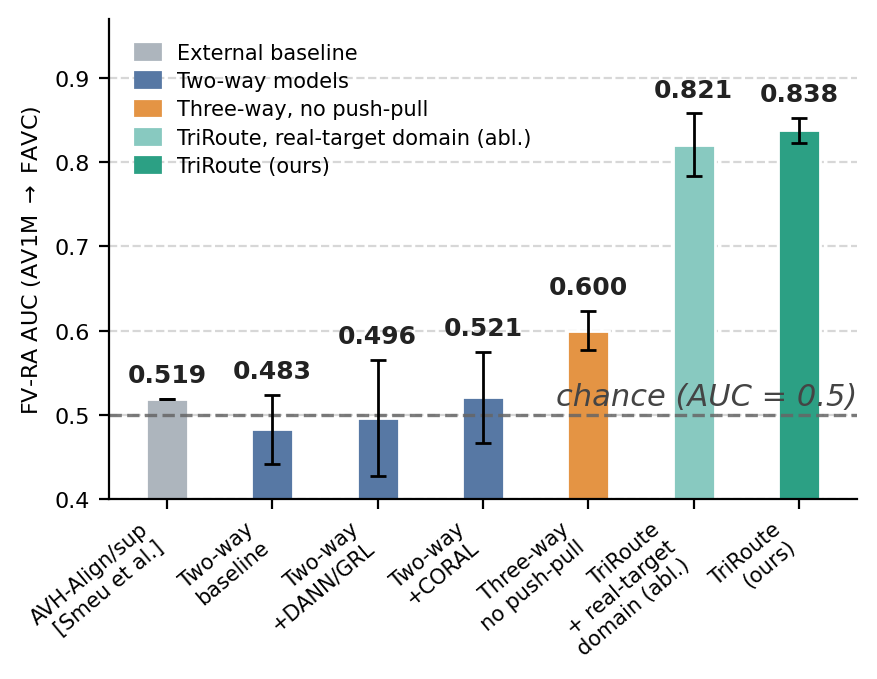
\includegraphics[width=\linewidth]{figures/fig_main_fvra.png}
    \caption{Cross-domain FV-RA AUC (AV1M $\to$ FAVC), mean over three seeds $\pm$1 std. Every two-way variant sits at or below chance; \method\ is the only model that clears $0.8$ AUC. Dashed line marks chance ($0.5$). This figure is the core empirical evidence that only TRIROUTE escapes the near-chance regime on FV-RA.}
    \label{fig:main_table_bar}
    \vspace{-5em}
\end{wrapfigure}


\paragraph{External baseline context.}
Table~\ref{tab:main} is primarily a mechanism table. The closest published AV1M-supervised baseline (AVH-Align/sup) shows the same FV-RA near-chance failure mode as our two-way baseline; the full category-level comparison is in Appendix~\ref{app:external_category}; protocol-matched comparison and artifact control are in Appendices~\ref{app:avhalign_protocol} and~\ref{app:artifact_control}.



Head-ablation results (Table~\ref{tab:ablation}, Figure~\ref{fig:head_ablation_delta}; full details in Appendix~\ref{app:head_ablation}) show that masking the visual-unique branch $u_v$ in \method\ drops FV-RA from $0.838$ to $0.491$ ($\Delta{=}{-}0.345$), while the same ablation on the two-way baseline causes only a negligible drop ($-0.034$)---an order-of-magnitude gap that is direct mechanism-level evidence of rerouting through the visual-unique factor. Additional branch-ablation evidence is provided in Appendix~\ref{app:head_ablation}.


\subsection{Qualitative Routing Examples}
Per-frame routing maps (Figure~\ref{fig:routing_map}) and representative FV-RA success/failure cases (Figures~\ref{fig:qualitative_success_appendix},~\ref{fig:qualitative_failure_appendix}) are provided in Appendix~\ref{app:qualitative_routing}.

\label{sec:qualitative}

% The aggregate diagnostics above quantify \emph{whether} the two-way baseline relies on the audio shortcut and \emph{whether} \method\ reroutes through visual evidence. To complement this with concrete cases, we mine FAVC FV-RA test clips on which the two-way baseline assigns very low fake probability ($P(\mathrm{fake}) < 0.5$) while \method\ assigns very high fake probability ($P(\mathrm{fake}) > 0.5$), and rank by score gap. Of $3{,}007$ FV-RA fake clips in the canonical FAVC test split, $1{,}048$ satisfy this ``two-way fails / \method\ corrects'' filter at seed~44, and the largest score gaps cluster tightly around $0.99$. Figure~\ref{fig:qualitative_main} shows one representative case: the audio waveform looks like ordinary speech (RealAudio is genuine for FV-RA), and the lip-region frames show the manipulated visual stream that the two-way baseline ignores. The two-way baseline assigns $P(\mathrm{fake}) \approx 0.01$ to this clip --- it is ``fooled'' by the genuine audio --- while \method\ assigns $P(\mathrm{fake}) \approx 1.00$. Five additional cases are shown in Figure~\ref{fig:qualitative_appendix} in the appendix, all drawn from the same top-gap pool and exhibiting the same pattern. Together with the head-ablation and input-perturbation evidence above, these cases illustrate the failure mode the three-way factorization is designed to prevent: when audio is real, a non-factorized detector has no incentive to use the visual stream, and confidently mislabels manipulated visual content as authentic.

% \begin{figure}[t]
%     \centering
%     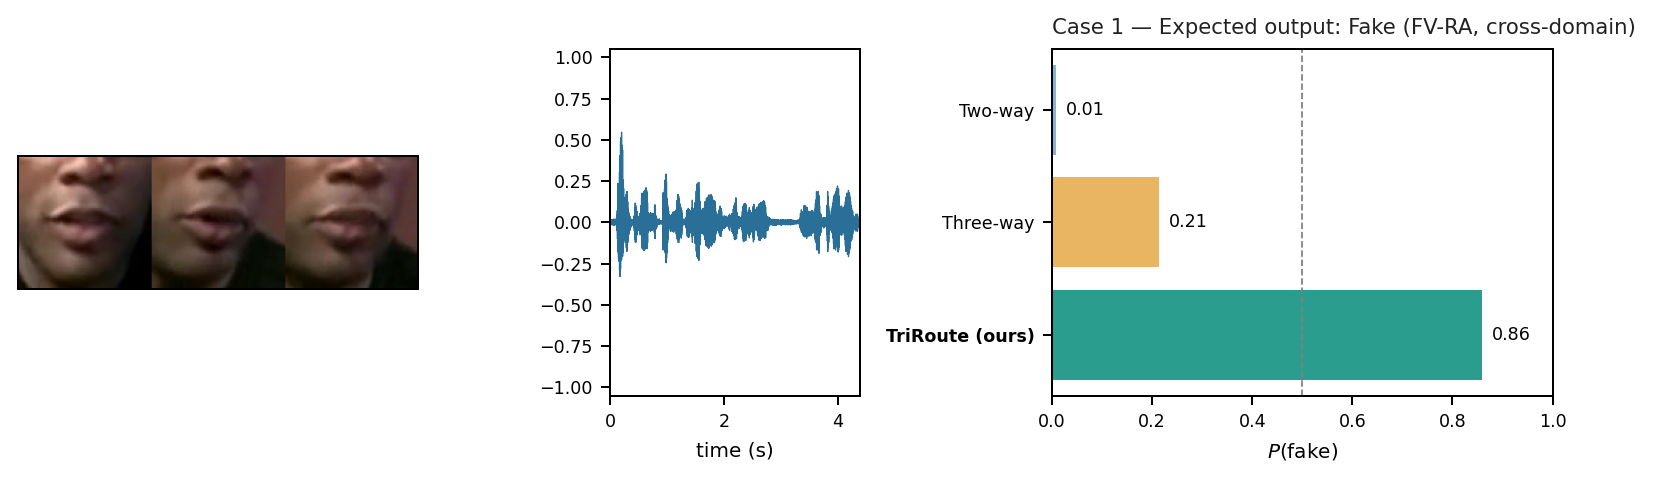
\includegraphics[width=0.97\linewidth]{fig_qualitative_main.png}
%     \caption{Representative FV-RA case where the two-way baseline misclassifies (follows the audio shortcut) and \method\ corrects (routes through the visual stream). \emph{Left:} three lip-region frames sampled across the clip, showing the manipulated visual stream. \emph{Middle:} the audio waveform; this is genuine RealAudio, which a non-factorized detector reads as evidence of authenticity. \emph{Right:} model fake-probabilities --- the two-way baseline assigns $P(\mathrm{fake}) \approx 0.01$, while \method\ assigns $P(\mathrm{fake}) \approx 1.00$. Five additional cases in Figure~\ref{fig:qualitative_appendix}.}
%     \label{fig:qualitative_main}
% \end{figure}

\subsection{Input-Level Routing Verification}
\label{sec:input_masking}
The head-ablation analysis zeroes out internal model components, which could conflate routing with capacity effects. As a complementary and model-agnostic test, we perturb the \emph{input features} on the FAVC FV-RA category and measure the resulting AUC change. This is a direct input-side intervention: if the trained head routes FV-RA decisions through the visual channel, full visual masking should cause a large drop; full audio masking, by contrast, should be neutral or beneficial (since FV-RA has real audio, masking it removes a potentially misleading signal).

Table~\ref{tab:perturbation} reports mean FV-RA AUC over three independent seeds at full audio masking ($p=1.0$) and full visual masking ($p=1.0$). Two patterns stand out. First, the two-way baseline barely changes under either masking ($\Delta_{\mathrm{audio}}=-0.021$, $\Delta_{\mathrm{visual}}=-0.077$), consistent with a model near chance on FV-RA that is not strongly routing through either modality. Second, the latest \method\ checkpoints show a strongly asymmetric profile: full visual masking lowers FV-RA from $0.838$ to $0.431$ on average ($\Delta=-0.407$), while full audio masking is approximately neutral ($\Delta=+0.005$). Three-way factorization without push-pull shows an intermediate profile ($\Delta_{\mathrm{audio}}=+0.040$, $\Delta_{\mathrm{visual}}=-0.137$), matching the intermediate FV-RA AUC in Table~\ref{tab:main}.

\begin{table}[t]
    \centering
    \caption{FV-RA AUC under full input masking on the FakeAVCeleb FV-RA category. Each row reports the mean over three independent seeds. $\Delta$ = masked AUC $-$ baseline AUC. A positive $\Delta_{\mathrm{audio}}$ indicates that removing the audio signal \emph{helps} FV-RA detection, i.e., the model is actively exploiting the visual channel and suppressing misleading real-audio signal. Baseline values should be interpreted within this intervention protocol; the relative ordering matches the main table.}
    \label{tab:perturbation}
    \small
    \begin{tabular}{lcccc}
        \toprule
        Model & Baseline & $\Delta_{\mathrm{audio}}$ (full) & $\Delta_{\mathrm{visual}}$ (full) & Relative visual sensitivity \\
        \midrule
        Two-way baseline        & $0.483$ & $-0.021$ & $-0.077$ & $1.0\times$ \\
        Three-way, no push-pull & $0.600$ & $+0.040$ & $-0.137$ & $1.8\times$ \\
        \method\ (ours) & $\mathbf{0.838}$ & $\mathbf{+0.005}$ & $\mathbf{-0.407}$ & $\mathbf{5.5\times}$ \\
        \bottomrule
    \end{tabular}
\end{table}

\paragraph{Progressive masking sweep (mechanism-level evidence).}
To go beyond the binary on/off intervention in Table~\ref{tab:perturbation}, we sweep the mask probability $p \in \{0, 0.1, 0.25, 0.5, 0.75, 1.0\}$ separately on the visual and audio channels, testing whether the FV-RA response degrades smoothly and monotonically. Figure~\ref{fig:masking_sweep} and Table~\ref{tab:masking_sweep} show that the curves are smooth and monotonic in the expected directions: visual masking lowers FV-RA AUC, audio masking raises it, and the magnitude of both effects grows from the two-way baseline through three-way (no push-pull) to \method. The two-way baseline is nearly flat under visual masking ($\Delta = -0.037$) and only mildly responsive to audio masking ($+0.095$), consistent with weak visual routing. \method\ shows the steepest visual-masking decline ($\Delta = -0.407$) and a clear positive response to audio masking ($+0.024$), indicating that the detector has learned to exploit visual evidence and tolerate or actively suppress real-audio distractors.


\begin{figure}[t]
    \centering
    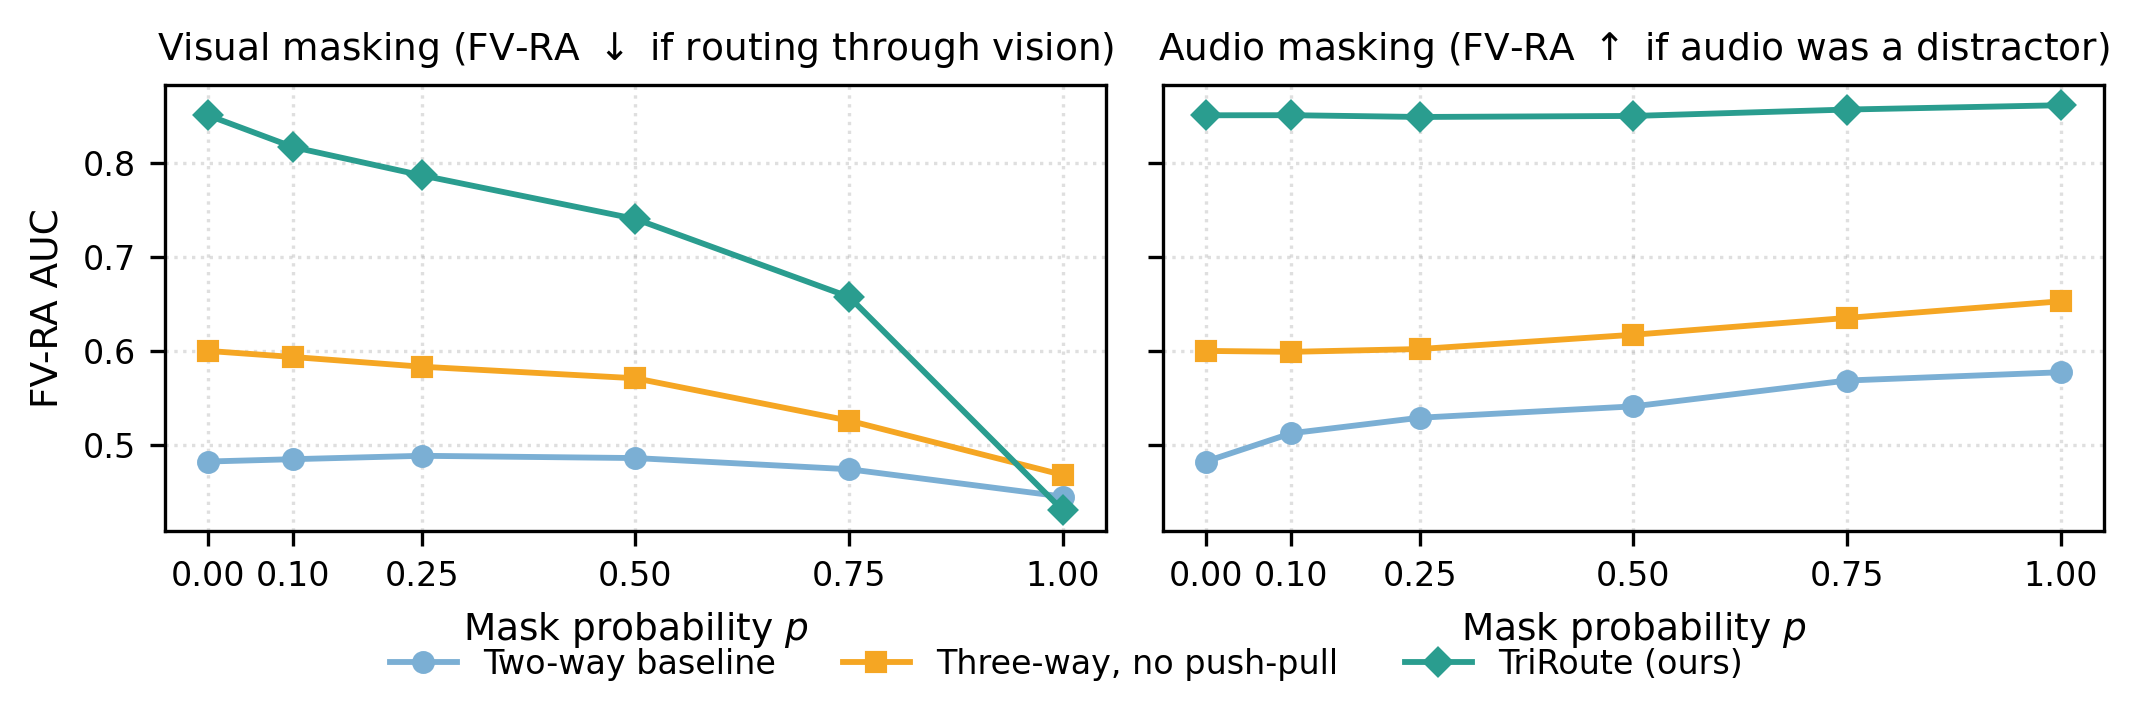
\includegraphics[width=0.97\linewidth]{figures/fig_masking_curves.png}
    \caption{Progressive input masking on FAVC FV-RA. \emph{Left:} visual masking monotonically lowers AUC, steepest for \method. \emph{Right:} audio masking monotonically raises AUC, as the real-audio stream is a distractor. The two-way baseline is nearly flat under visual masking (weak visual routing).}
    \label{fig:masking_sweep}
\end{figure}

\begin{table}[t]
    \centering
    \caption{Progressive input masking on FAVC FV-RA AUC. Top block: visual masking ($\Delta < 0$ indicates visual routing). Bottom block: audio masking ($\Delta > 0$ indicates audio was a distractor). Numbers correspond to Figure~\ref{fig:masking_sweep}. Baseline values at $p{=}0.0$ differ from Table~\ref{tab:main} because the masking-sweep evaluation uses a separate run; the relative ordering across models is preserved.}
    \label{tab:masking_sweep}
    \small
    \begin{tabular}{lccccccc}
        \toprule
        Model & $p{=}0.0$ & $p{=}0.1$ & $p{=}0.25$ & $p{=}0.5$ & $p{=}0.75$ & $p{=}1.0$ & $\Delta(0{\rightarrow}1)$ \\
        \midrule
        \multicolumn{8}{l}{\emph{Visual masking}} \\
        Two-way baseline        & $0.483$ & $0.485$ & $0.489$ & $0.486$ & $0.474$ & $0.445$ & $-0.037$ \\
        Three-way, no push-pull & $0.600$ & $0.594$ & $0.584$ & $0.571$ & $0.526$ & $0.468$ & $-0.132$ \\
        \method\ (ours)         & $0.838$ & $0.817$ & $0.787$ & $0.741$ & $0.658$ & $0.431$ & $\mathbf{-0.407}$ \\
        \midrule
        \multicolumn{8}{l}{\emph{Audio masking}} \\
        Two-way baseline        & $0.483$ & $0.513$ & $0.529$ & $0.541$ & $0.569$ & $0.578$ & $\mathbf{+0.095}$ \\
        Three-way, no push-pull & $0.600$ & $0.599$ & $0.602$ & $0.618$ & $0.635$ & $0.653$ & $+0.053$ \\
        \method\ (ours)         & $0.838$ & $0.841$ & $0.849$ & $0.850$ & $0.857$ & $0.862$ & $+0.024$ \\
        \bottomrule
    \end{tabular}
\end{table}

\subsection{Subspace Probe Analysis}
\label{sec:subspace_probe}

Subspace probing results are in Appendix~\ref{app:subspace_probe} (Table~\ref{tab:subspace_probe}, Figures~\ref{fig:subspace_probe} and~\ref{fig:tsne}). The key finding: the visual-unique factor $u_v$ achieves $0.924$ OOD FV-RA probe AUC in just $256$ dimensions, higher than the full $1024$-dim two-way representation ($0.705$), while domain probe AUC remains high ($0.976$) across all subspaces---routing rather than domain invariance.

\subsection{Unsupervised Scaling Stress Test}
\label{sec:scaling_stress}

We tested whether simply increasing the amount of unsupervised pretraining data recovers the FV-RA routing behavior. Full results are reported in Appendix~\ref{app:scaling_stress}. In short, scaling unsupervised training to 250K clips does not approach the FV-RA AUC achieved by structural factorization ($0.838$), supporting the conclusion that the bottleneck is routing structure, not data quantity.

\section{Limitations and Broader Impact}
\paragraph{Limitations.}
\method\ is anchored to speech-related evidence and may underperform on deepfakes with minimal lip motion or absent audio. The category-level gain is concentrated in FV-RA, because RV-FA and FV-FA are near ceiling; this limits how broadly the result generalises across manipulation categories. The baseline comparison is mechanism-oriented rather than an exhaustive leaderboard: we compare against AVH-Align/sup and internal ablation controls, but do not retrain AVAD, SpeechForensics, or AVFF under the same protocol. The factorization requires some nuisance partition during training; whether stronger or multi-source domain contrast yields further gains is open. Finally, the routing evidence is mechanistic rather than a formal causal proof: future work should vary the capacity of $u_v$ and the residual branch directly.

\paragraph{Broader impact.}
Cross-domain deepfake detection can support content authentication, media forensics, and platform integrity. At the same time, any detector can be misused for surveillance or overconfident moderation, especially if its uncertainty is not surfaced. We therefore recommend reporting calibration, failure modes, and domain-shift sensitivity, and releasing models with clear usage restrictions and dataset documentation.


\section{Conclusion}

Cross-domain audio-visual deepfake detection poses a specific routing problem: models trained on source data learn to exploit audio correlates of the fake label, and when those correlates break at test time---as in the FV-RA category, where the audio stream is genuine---performance collapses near chance. Standard remedies do not resolve this. Domain-adversarial training and covariance alignment reduce domain discrepancy globally, but applied to entangled two-way representations they leave the classifier free to route decisions through whichever branch is most convenient. The audio branch remains the easiest path, and without a structural constraint, the classifier continues to take it.

\method\ addresses this by design rather than by penalty. Decomposing frozen AV-HuBERT features into shared content $(s_v, s_a)$, modality-unique manipulation factors $(u_v, u_a)$, and a residual branch $(r_v, r_a)$ that is explicitly trained to absorb domain-correlated nuisance and then excluded from the prediction head removes the shortcut as a usable option rather than merely discouraging it. A push-pull objective reinforces this: $\mathcal{L}_{\mathrm{dom}}$ attracts domain signal into the residual branch, while $\mathcal{L}_{\mathrm{adv}}$ makes easy domain prediction from the task branch adversarially difficult, so that routing through genuine visual manipulation evidence becomes the path of least resistance.

On the AV1M$\rightarrow$FAVC benchmark, this structural design yields $0.838$ FV-RA AUC using only source-side speaker-group nuisance labels---a $+0.319$ improvement over AVH-Align/sup ($0.519$), the closest published baseline trained on the same source data, and a $+0.238$ improvement over three-way factorization without the push-pull objective ($0.600$), isolating the contribution of the domain objectives above and beyond structure alone. The two objective-level controls on the same two-way representation---DANN/GRL ($0.496$) and CORAL ($0.521$)---neither clears chance on FV-RA, confirming that the bottleneck is architectural rather than loss-level. The ordering is preserved on a second external benchmark, AVLips ($0.789$ vs.\ $0.533$ for the two-way baseline), indicating that the gain generalises beyond a single target dataset.

Three independent lines of evidence confirm that the gains reflect a change in inference-time routing rather than stronger representations or better regularisation. \emph{Head ablation}: masking the visual-unique factor $u_v$ drops \method's FV-RA from $0.838$ to $0.491$, a $-0.345$ fall that is an order of magnitude larger than the same ablation on the two-way baseline ($-0.034$). \emph{Input masking}: zeroing the visual input collapses \method's FV-RA by $0.407$, while zeroing the audio stream is approximately neutral ($+0.005$)---the detector actively exploits visual evidence and treats real-audio as a distractor rather than a cue. \emph{Subspace probing}: the $256$-dim visual-unique factor $u_v$ achieves $0.924$ OOD FV-RA probe AUC, exceeding the full $1024$-dim two-way representation ($0.705$), while domain identity remains decodable at high accuracy from every subspace. Domain information is not erased; it is displaced away from the prediction pathway.

Together, these results point to a reframing of the core challenge: the bottleneck in cross-domain multimodal deepfake detection is not the absence of stronger objectives or more data, but the absence of structural constraints on the prediction pathway. Giving shortcut signals a dedicated branch---and excluding that branch from the classifier head---forces the model to route through genuine manipulation evidence. Explicitly controlling which information a model is \emph{allowed to use} may be a more reliable foundation for robustness than attempting to remove spurious signals from representations.

\bibliographystyle{plainnat}
\bibliography{references}

\newpage
\appendix
\section{Implementation Details (Extended)}
\label{app:implementation_details}

\paragraph{Nuisance label derivation.}
Nuisance labels are derived entirely from the AV1M training set via a speaker-group hash ($d = \mathrm{hash}(\mathrm{speaker\_id})\bmod 2$), assigning all clips of a speaker to the same binary group; no FakeAVCeleb data enters training, validation, or model selection. This is deliberately weaker than true target-domain supervision and should be understood as a source-side nuisance partition. Unless otherwise stated, quantitative results report the mean over three independent seeds.
\paragraph{Batch size and gradient accumulation.}
All models are trained with batch size~1 (one clip per gradient step). This choice is imposed by the variable sequence length of AV-HuBERT features: each clip produces a different number of frames $T$, so a fixed-shape batch tensor cannot be constructed without padding. Rather than pad-and-mask (which would require re-implementing the temporal alignment loss), we process one clip at a time. No gradient accumulation is used: the alignment loss $\mathcal{L}_{\mathrm{align}}$ operates within a single clip's temporal window and does not benefit from cross-clip accumulation. The resulting per-step gradient is therefore a single-sample stochastic estimate, which is noisier than a mini-batch gradient but consistent across all model variants in the ablation table. All baselines (DANN/GRL, CORAL, two-way, three-way no push-pull) use the same batch size~1 setting for a fair comparison.

\paragraph{Matched settings for DANN/CORAL controls.}
For fairness, the DANN/GRL and CORAL controls use matched optimization settings (Adam $10^{-3}$, GRL $\alpha{=}1.0$, CORAL weight $\lambda{=}1.0$) under the same seed/checkpoint policy. We do not perform target-aware tuning sweeps on FakeAVCeleb labels.

\paragraph{Compute.}
All supervised models are trained from pre-extracted frozen AV-HuBERT features; the reported detector training cost therefore excludes AV-HuBERT pretraining. Each training run uses a single GPU from the university HPC cluster, 4 CPU workers, and 32\,GB host memory. The primary partition used for the main \method\ runs and the DANN/GRL sweep is \textbf{NVIDIA A100 PCIe} (40\,GB); some auxiliary runs use NVIDIA L40S (48\,GB) depending on queue availability. A 100-epoch \method\ run completes in approximately \textbf{5.5\,hours}; the three-seed headline result requires ${\approx}16.5$\,GPU-hours (${\approx}0.7$\,GPU-days). The full main-table comparison (six model variants, three seeds each) costs ${\approx}63$\,GPU-hours (${\approx}4.1$\,GPU-days) for training.

\paragraph{Seed policy.}
All model families in the main ablation table are reported as means over three independent seeds under the same source-validation checkpointing rule. We do not select checkpoints or seeds using FakeAVCeleb labels.

\section{External Baseline Category Comparison}
\label{app:external_category}

The AV1M-trained AVH-Align/sup checkpoint from \citet{smeu2025avhalign} is the most directly comparable published supervised baseline. As Table~\ref{tab:external_category} shows, it exhibits the same category-level failure mode as our two-way baseline: RV-FA and FV-FA are near ceiling, while FV-RA remains near chance ($0.519$). \method's FV-RA gain therefore addresses the visual-fake transfer failure of the closest published supervised baseline, not only our internal ablations.

\begin{table}[h]
    \centering
    \caption{Category-level external supervised baseline on FakeAVCeleb (AV1M $\to$ FAVC). AVH-Align/sup is the AV1M-trained supervised checkpoint from \citet{smeu2025avhalign}, evaluated with the same category protocol as Table~\ref{tab:main}. Values are AUC/AP.}
    \label{tab:external_category}
    \small
    \begin{tabular}{lcccc}
        \toprule
        Method & Overall & RV-FA & FV-RA & FV-FA \\
        \midrule
        AVH-Align/sup \citep{smeu2025avhalign} & $0.777/0.994$ & $0.999/0.999$ & $0.519/0.955$ & $0.999/1.000$ \\
        \method\ (ours) & $\mathbf{0.922/0.998}$ & $0.999/0.999$ & $\mathbf{0.838/0.989}$ & $0.994/1.000$ \\
        \bottomrule
    \end{tabular}
\end{table}

\section{Head-Ablation Details}
\label{app:head_ablation}

Table~\ref{tab:ablation} and Figure~\ref{fig:head_ablation_delta} quantify how strongly each model's FV-RA performance depends on its visual branches. For the two-way baseline, zeroing the visual task branch causes a negligible drop of $-0.034$, confirming that the trained detector barely uses visual evidence for FV-RA decisions. For three-way factorization without domain push-pull, masking visual branches causes a larger drop ($-0.113$), indicating partial visual usage. In the latest \method\ checkpoints, mean FV-RA falls from $0.838$ to $0.491$ when $u_v$ is masked and to $0.441$ when both visual branches are masked. The order-of-magnitude gap ($-0.034$ vs.\ $-0.345$) is mechanism-level evidence that \method\ has rerouted FV-RA decisions through the visual-unique factor. Masking the audio branch of the two-way baseline instead drops in-domain AUC from $0.997$ to $0.528$, confirming audio dominance rather than visual capacity failure.

\begin{table}[h]
    \centering
    \caption{Head-ablation analysis on FV-RA AUC. Each row zeros out one branch of the trained model and measures the FV-RA drop ($\Delta$FV-RA). Larger drop indicates heavier routing dependence on that branch. All rows report the mean over three independent seeds.}
    \label{tab:ablation}
    \resizebox{\linewidth}{!}{%
    \begin{tabular}{llccc}
        \toprule
        Model & Ablation & Baseline FV-RA & Ablated FV-RA & $\Delta_{\mathrm{FV\text{-}RA}}$ \\
        \midrule
        Two-way baseline & mask visual task branch & $0.495$ & $0.461$ & $-0.034$ \\
        Three-way, no domain push-pull & mask visual branches & $0.586$ & $0.473$ & $-0.113$ \\
        \method\ (ours) & mask manipulation ($u_v$) & $\mathbf{0.838}$ & $0.491$ & $\mathbf{-0.345}$ \\
        \method\ (ours) & mask visual branches & $\mathbf{0.838}$ & $0.441$ & $\mathbf{-0.395}$ \\
        \bottomrule
    \end{tabular}}
\end{table}

\begin{figure}[h]
    \centering
    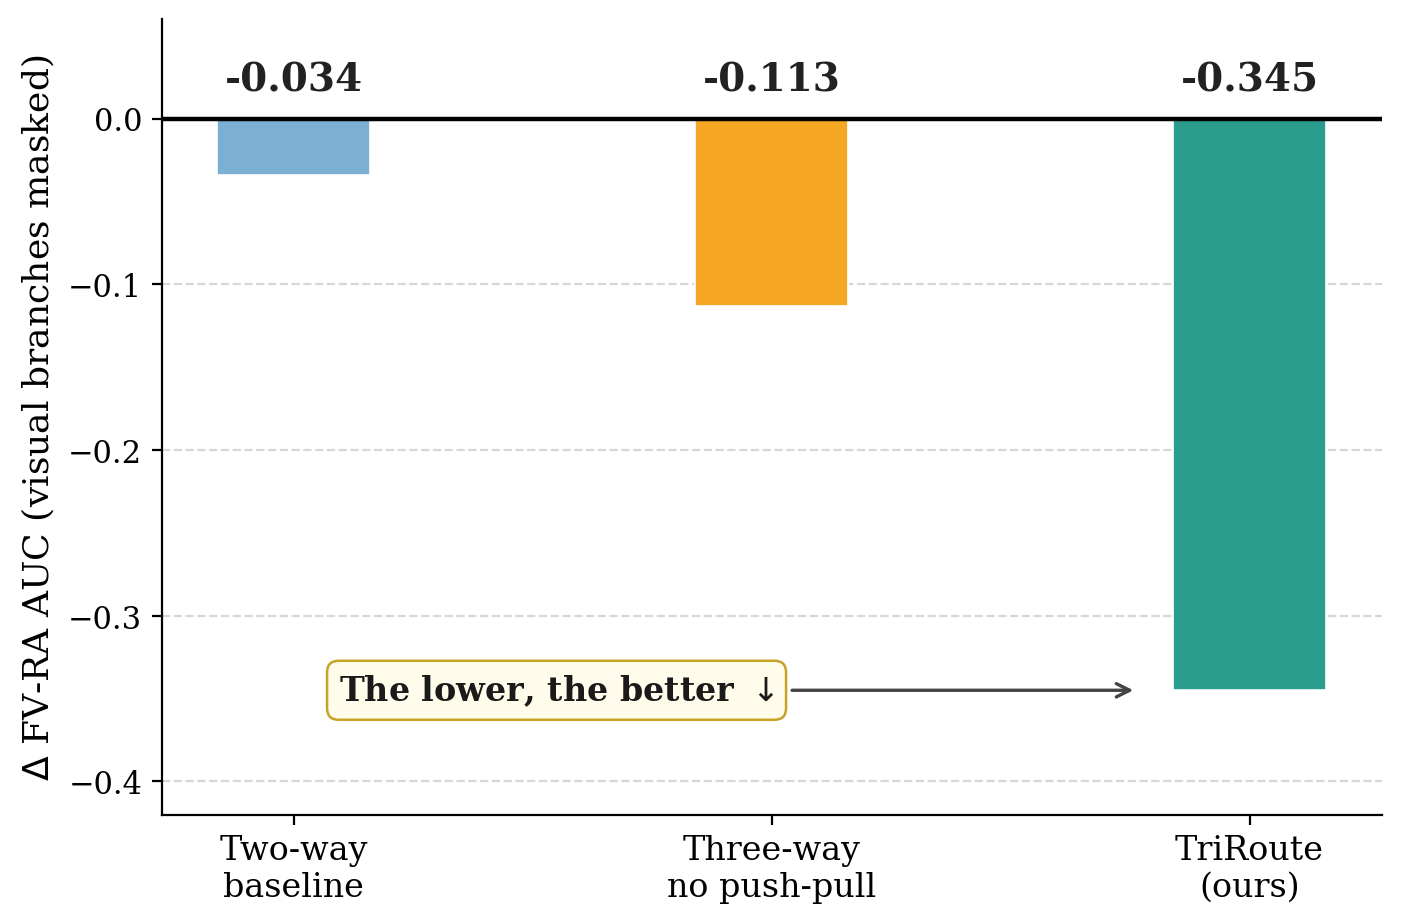
\includegraphics[width=0.55\linewidth]{figures/fig_head_ablation_delta.png}
    \caption{Head-ablation routing dependence on the visual branches, summarising Table~\ref{tab:ablation}. Each bar is the magnitude of the FV-RA AUC drop when visual branches are masked. Only the factorized \method\ model is meaningfully sensitive to removing visual components: the drop is roughly an order of magnitude larger than the two-way baseline ($-0.345$ vs.\ $-0.034$).}
    \label{fig:head_ablation_delta}
\end{figure}

\section{Qualitative Routing and Per-Frame Routing Maps}
\label{app:qualitative_routing}

Figure~\ref{fig:routing_map} shows per-frame routing maps for representative FAVC FV-RA clips. For fake clips, the visual-unique factor $\|u_v^t\|$ shows sharp peaks aligned with manipulation events; for real clips, it stays low while the residual carries the bulk of the activation. The prediction head reads only $u_v$ (and $s_v$), so the asymmetry in $\|u_v^t\|$ between the two clips drives the score. Of $3{,}007$ FV-RA fake clips in the canonical FAVC test split, $1{,}048$ satisfy the ``two-way fails / \method\ corrects'' filter at seed~44, and the largest score gaps cluster around $0.99$. Additional success and failure cases are in Figures~\ref{fig:qualitative_success_appendix} and~\ref{fig:qualitative_failure_appendix} (Appendix~\ref{app:qualitative}).

\begin{figure}[h]
    \centering
    
\includegraphics[width=0.95\linewidth]{figures/routing_map.pdf}
    \caption{Per-frame routing map for two FAVC clips classified by \method. We plot the time-varying feature norm of the visual-unique factor $\|u_v^t\|$ (solid blue) and the residual factor $\|r_v^t\|$ (dashed orange). \emph{Top:} a correctly classified fake (FV-RA) clip --- $\|u_v^t\|$ has sharp peaks aligned with manipulation events. \emph{Bottom:} a correctly classified real clip --- $\|u_v^t\|$ stays low while the residual carries the bulk of the activation.}
    \label{fig:routing_map}
\end{figure}

\section{Subspace Probe Analysis}
\label{app:subspace_probe}

To check that the structural separation concentrates transferable visual evidence into a specific component, we train light linear probes directly on individual subspaces and report cross-domain (OOD) FV-RA AUC and domain-classification AUC. A useful manipulation pathway should be predictive of FV-RA \emph{and} relatively domain-blind.

\begin{table}[h]
    \centering
    \caption{Subspace probe analysis. Linear probes are trained on each subspace and evaluated for cross-domain FV-RA AUC and domain-classification AUC. The visual-unique factor $u_v$ in \method\ achieves the strongest cross-domain probe AUC despite having only $256$ dimensions.}
    \label{tab:subspace_probe}
    \small
    \begin{tabular}{llcc}
        \toprule
        Model & Subspace (Dim.) & OOD probe AUC & Domain probe AUC \\
        \midrule
        Two-way & task branch $Z_c$ ($1024$)        & $0.705$ & $0.998$ \\
        Two-way & visual factor $v_c$ ($512$)       & $0.891$ & $0.994$ \\
        Three-way, no push-pull & shared visual $s_v$ ($256$)  & $0.814$ & $0.992$ \\
        Three-way, no push-pull & unique visual $u_v$ ($256$)  & $0.825$ & $0.967$ \\
        \method\ (ours) & shared visual $s_v$ ($256$)  & $0.726$ & $0.989$ \\
        \method\ (ours) & unique visual $u_v$ ($256$)  & $\mathbf{0.924}$ & $0.976$ \\
        \bottomrule
    \end{tabular}
\end{table}

\begin{figure}[h]
    \centering
    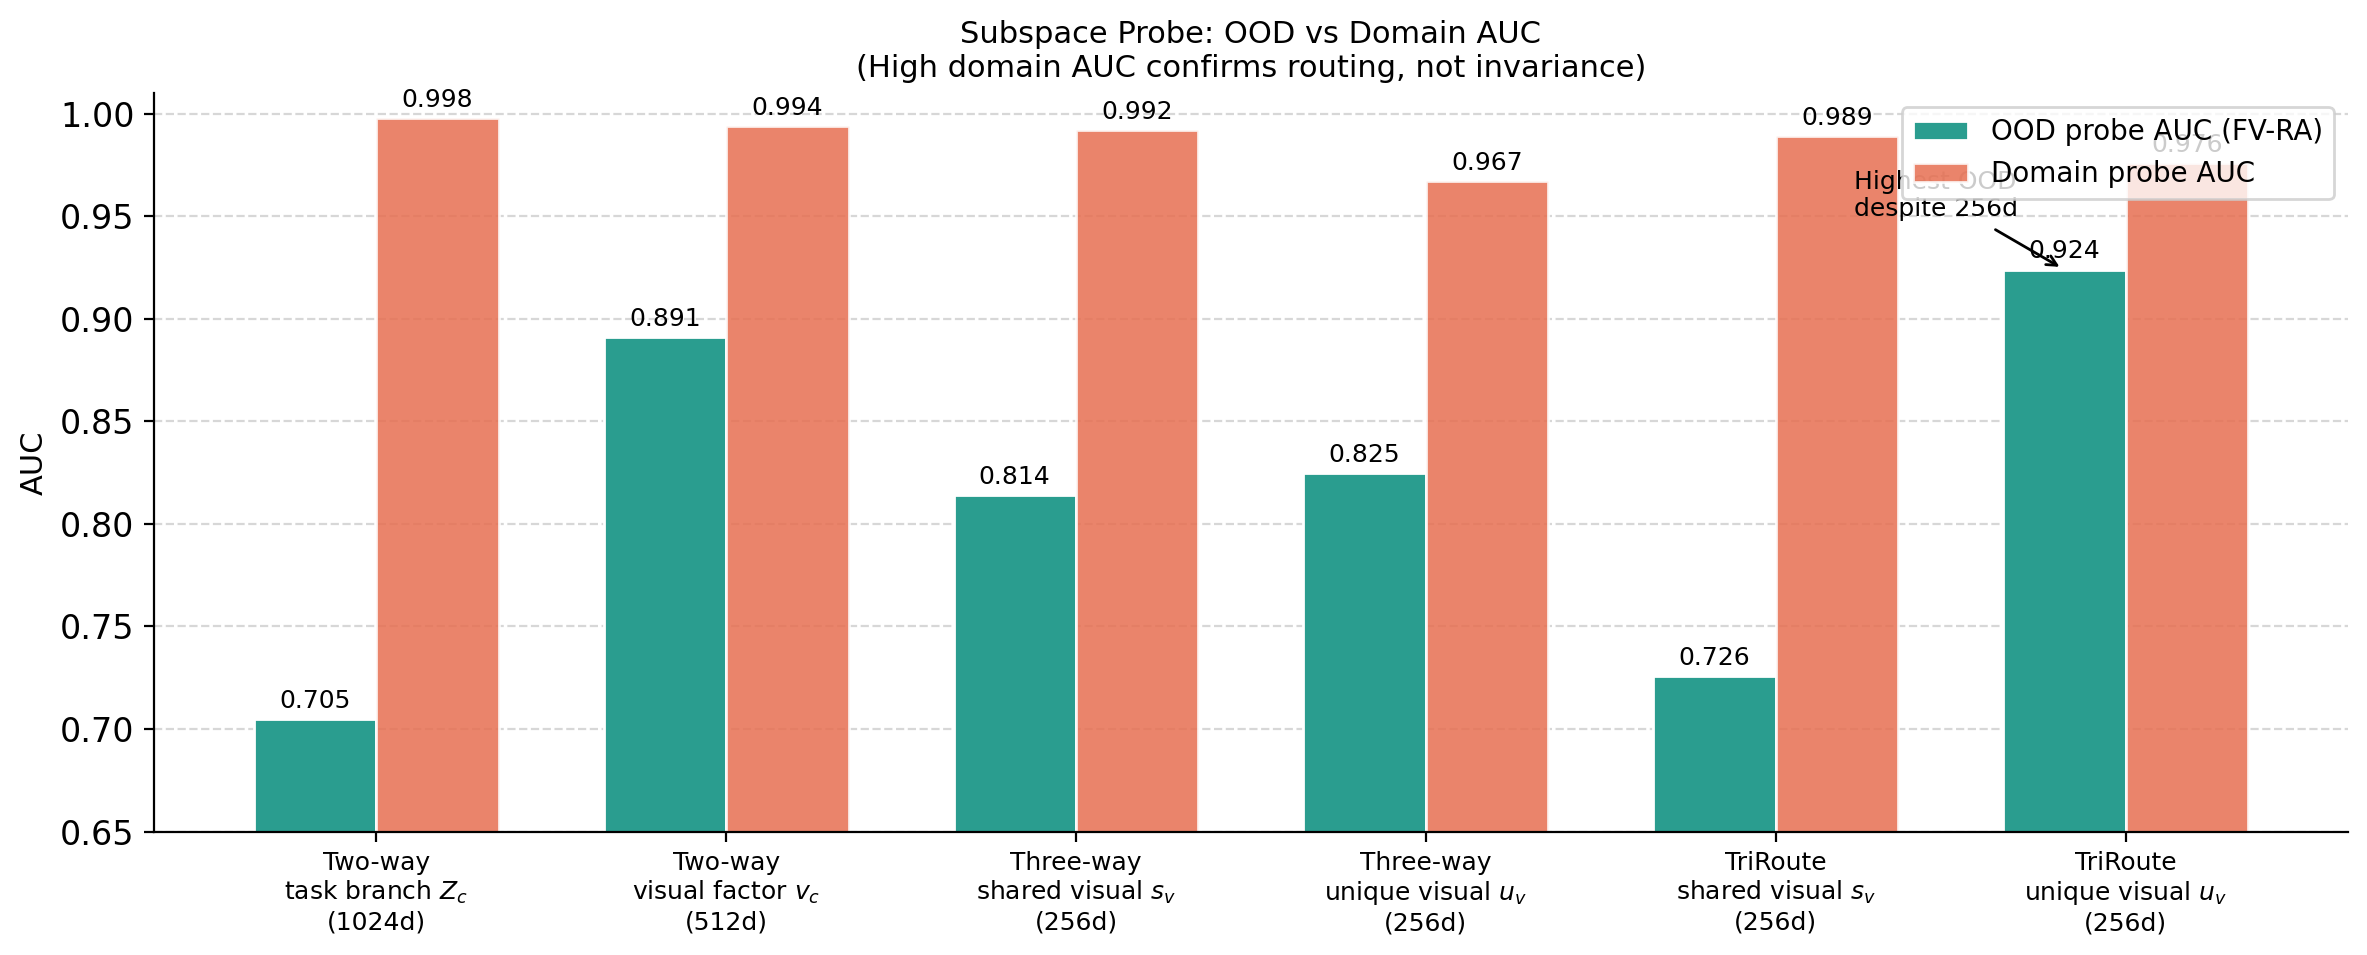
\includegraphics[width=0.97\linewidth]{figures/fig_subspace_probe.png}
    \caption{Subspace probe AUCs for OOD FV-RA prediction (teal) and domain prediction (orange) across the six subspaces in Table~\ref{tab:subspace_probe}. The visual-unique factor $u_v$ in \method\ achieves the strongest cross-domain probe AUC ($0.924$) at only $256$ dimensions, while the domain probe stays high ($0.976$) across all subspaces---routing rather than invariance.}
    \label{fig:subspace_probe}
\end{figure}

The $256$-dim $u_v$ attains $0.924$ OOD probe AUC, higher than both the $1024$-dim fused two-way representation ($0.705$) and the $512$-dim two-way visual factor ($0.891$)---higher OOD performance despite lower dimensionality. The domain-classification probe stays high on every subspace ($0.967$--$0.998$): domain identity is not erased but displaced away from the prediction-relevant subspace, consistent with the push-pull objective. Figure~\ref{fig:tsne} provides a qualitative complement.

\begin{figure}[h]
    \centering
    
\includegraphics[width=0.95\linewidth]{figures/tsne.png}
    \caption{t-SNE projections of \method's residual and manipulation factors on held-out clips from AV-Deepfake1M, FakeAVCeleb, and AVLips. \emph{Left:} the residual factor cleanly separates source and target datasets, confirming domain-correlated nuisance is concentrated in the structurally excluded branch. \emph{Right:} the manipulation factor separates real from fake regardless of dataset, indicating the prediction-relevant subspace generalizes across domains.}
    \label{fig:tsne}
\end{figure}
\section{Multi-Seed Results and Prepared Sweeps}
\label{app:seed_and_sweeps}

Table~\ref{tab:raw_seed_results} reports multi-seed mean~$\pm$~std for the completed FAVC 70/30 baseline sweep. Std is the sample standard deviation (denominator $n-1$).

\begin{table}[h]
    \centering
    \caption{FAVC 70/30 AUC multi-seed mean~$\pm$~std for the baseline sweep. FV-RA is the visual-routing diagnostic.}
    \label{tab:raw_seed_results}
    \small
    \begin{tabular}{lcccc}
        \toprule
        Model & Overall & RV-FA & \textbf{FV-RA} & FV-FA \\
        \midrule
        Two-way baseline & $0.760\pm0.020$ & $1.000\pm0.000$ & $\mathbf{0.483\pm0.041}$ & $0.998\pm0.002$ \\
        Three-way, no push-pull & $0.827\pm0.024$ & $1.000\pm0.000$ & $\mathbf{0.600\pm0.022}$ & $0.998\pm0.001$ \\
        \method\ (ours) & $0.922\pm0.041$ & $1.000\pm0.000$ & $\mathbf{0.838\pm0.087}$ & $0.997\pm0.002$ \\
        \bottomrule
    \end{tabular}
\end{table}

\paragraph{Hyperparameter sensitivity.}
Table~\ref{tab:sensitivity_sweep} reports a one-at-a-time sensitivity audit of the three domain-routing loss weights. Each row holds two weights fixed at their defaults ($\lambda_{\mathrm{dom}}{=}1.0$, $\lambda_{\mathrm{adv}}{=}1.0$, $\lambda_{\mathrm{ortho}}{=}0.1$) and varies the third; all runs use three multiple seeds and the same source-validation checkpointing rule with no FAVC labels. Two observations stand out. First, the default setting is at or near the optimum of each one-dimensional sweep, indicating that it was not adversarially tuned. Second, and more importantly, even the worst single configuration in the sweep ($\lambda_{\mathrm{adv}}{=}3.0$, FV-RA $0.682$) remains $+0.168$ above the best mean FV-RA of the DANN/GRL baseline across its own $\alpha$-sweep ($0.514$, Table~\ref{tab:dann_alpha_sweep}). The routing gain is therefore not explained by lucky default weight choices: it is present across the entire range tested.

\begin{table}[h]
    \centering
    \caption{One-at-a-time loss-weight sensitivity on FAVC FV-RA AUC. Default values: $\lambda_{\mathrm{dom}}{=}1.0$, $\lambda_{\mathrm{adv}}{=}1.0$, $\lambda_{\mathrm{ortho}}{=}0.1$. The default row is shaded; all other rows vary exactly one weight. The DANN/GRL best mean FV-RA is $0.514$ (Table~\ref{tab:dann_alpha_sweep}).}
    \label{tab:sensitivity_sweep}
    \small
    \begin{tabular}{ccc|c}
        \toprule
        $\lambda_{\mathrm{dom}}$ & $\lambda_{\mathrm{adv}}$ & $\lambda_{\mathrm{ortho}}$ & \textbf{FV-RA AUC} \\
        \midrule
        $0.3$ & $1.0$ & $0.1$ & $0.773$ \\
        \rowcolor[gray]{0.92} $1.0$ & $1.0$ & $0.1$ & $\mathbf{0.838}$ \\
        $3.0$ & $1.0$ & $0.1$ & $0.722$ \\
        \midrule
        $1.0$ & $0.3$ & $0.1$ & $0.763$ \\
        $1.0$ & $3.0$ & $0.1$ & $0.682$ \\
        \midrule
        $1.0$ & $1.0$ & $0.03$ & $0.745$ \\
        $1.0$ & $1.0$ & $0.3$  & $0.754$ \\
        \bottomrule
    \end{tabular}
\end{table}

\paragraph{DANN/GRL strength audit.}
The DANN baseline audit uses the same code path as the main DANN row and sweeps $\alpha \in \{0.1,0.3,0.5,1.0,3.0\}$ across seeds $\{43,44,45\}$. Table~\ref{tab:dann_alpha_sweep} shows that increasing or decreasing the GRL strength does not close the visual-routing gap: the best mean FV-RA AUC is $0.514$ at $\alpha=0.3$, and even the strongest single run in the sweep ($\alpha=3.0$, seed~43, FV-RA AUC $0.601$) remains far below \method's $0.838$. Thus the weak DANN result is not explained by an unlucky default $\alpha$.

\begin{table}[h]
    \centering
    \caption{DANN/GRL strength sweep on FakeAVCeleb 70/30. Each row reports mean AUC over three seeds. Std. is the sample standard deviation over seeds for FV-RA AUC.}
    \label{tab:dann_alpha_sweep}
    \small
    \begin{tabular}{lccc}
        \toprule
        GRL $\alpha$ & Overall AUC & \textbf{FV-RA AUC} & FV-RA std. \\
        \midrule
        $0.1$ & $0.757$ & $0.475$ & $0.007$ \\
        $0.3$ & $\mathbf{0.775}$ & $\mathbf{0.514}$ & $0.033$ \\
        $0.5$ & $0.758$ & $0.479$ & $0.014$ \\
        $1.0$ & $0.755$ & $0.473$ & $0.028$ \\
        $3.0$ & $0.771$ & $0.509$ & $0.083$ \\
        \bottomrule
    \end{tabular}
\end{table}

\section{Domain Label Quality}
\label{app:domain_label_quality}

A natural question is how much the quality of nuisance supervision matters. The speaker-group pseudo-label is not a target-domain label: it partitions source clips by speaker identity and is therefore closer to a weak speaker-group nuisance proxy than to true knowledge of the AV1M-to-FAVC domain gap. It does not directly encode codec differences, acquisition conditions, or any FAVC-specific artifact. Yet the latest \method\ checkpoints raise FV-RA AUC from the two-way baseline of $0.483$ to $0.838$, a $+0.355$ gain without using any FakeAVCeleb data during training. We therefore interpret nuisance supervision as helpful but secondary to the representation split itself: even a weak source-side partition is enough to make the residual sink useful once the classifier is structurally prevented from reading it.

\section{Comparison in AVH-Align Protocol}
\label{app:avhalign_protocol}

Table~\ref{tab:avhalign_comparison} replicates the structure of Table~2 in \citet{smeu2025avhalign}, reporting AUC and AP on the FakeAVCeleb 70/30 test split and AV-Deepfake1M validation set ($N=2{,}000$), with and without leading-silence trimming. Baseline rows are reproduced from \citet{smeu2025avhalign}. Our rows report the source-side nuisance-label variant averaged over three independent seeds. The most direct comparison is the supervised AV1M-trained AVH-Align row; after leading-silence trimming, \method\ remains clearly stronger on FAVC ($86.6$ vs.\ $70.8$ AUC). The unsupervised VoxCeleb2-pretrained rows are included for context rather than as matched baselines.
Note that \method\ trained directly on FAVC reaches near-ceiling in-domain performance (AUC $99.6$, lower block of Table~\ref{tab:avhalign_comparison}), indicating that the AV1M$\rightarrow$FAVC gap is not a model-capacity limitation of \method\ but a manifestation of cross-dataset shift.

\begin{table}[h]
    \centering
    \caption{Protocol context: this table is not a headline leaderboard. Comparison with \citet{smeu2025avhalign} Table~2 baselines on FakeAVCeleb (FAVC) 70/30 test split and AV-Deepfake1M (AV1M) validation set. Values are percentages. Trim:$\checkmark$ denotes leading-silence-trimmed evaluation. Baseline rows are reproduced from \citet{smeu2025avhalign}; the headline supervised and unsupervised rows report the mean over three independent seeds. \textbf{Bold} = best, \underline{underline} = second best within each training-data block. FAVC-trained rows show the reverse-direction transfer. The post-hoc fusion row is in Appendix~\ref{app:posthoc_fusion}.}
    \label{tab:avhalign_comparison}
    \resizebox{\linewidth}{!}{%
    \begin{tabular}{llllcccccccc}
        \toprule
        & & & & \multicolumn{4}{c}{Metric: AUC} & \multicolumn{4}{c}{Metric: AP} \\
        \cmidrule(lr){5-8}\cmidrule(lr){9-12}
        & & & & \multicolumn{2}{c}{FakeAVCeleb} & \multicolumn{2}{c}{AV-Deepfake1M} & \multicolumn{2}{c}{FakeAVCeleb} & \multicolumn{2}{c}{AV-Deepfake1M} \\
        \cmidrule(lr){5-6}\cmidrule(lr){7-8}\cmidrule(lr){9-10}\cmidrule(lr){11-12}
        Method & Mod. & Train type & Train data & Trim:$\times$ & Trim:$\checkmark$ & Trim:$\times$ & Trim:$\checkmark$ & Trim:$\times$ & Trim:$\checkmark$ & Trim:$\times$ & Trim:$\checkmark$ \\
        \midrule
        \multicolumn{12}{l}{\emph{Unsupervised pretraining (reproduced from \citet{smeu2025avhalign})}} \\
        AVAD \citep{feng2023avad}               & AV & unsup. & LRS       & 84.5 & 84.7 & 54.3 & 54.3 & \underline{99.5} & \underline{99.5} & 76.3 & 76.3 \\
        SpeechForensics \citep{liang2024speechforensics} & AV & unsup. & VoxCeleb2 & \textbf{98.8} & \textbf{98.8} & 68.8 & 68.2 & \textbf{100.0} & \textbf{100.0} & 83.7 & 83.5 \\
        AVH-Align \citep{smeu2025avhalign}      & AV & unsup. & VoxCeleb2 & \underline{94.6} & \underline{94.6} & \textbf{85.9} & \textbf{83.5} & \underline{99.8} & \underline{99.8} & \textbf{94.3} & \textbf{93.5} \\
        \method\ (unsup, ours)                  & AV & unsup. & VoxCeleb2 & 93.1 & 92.8 & \underline{85.4} & \underline{82.1} & 99.5 & 99.5 & \underline{90.9} & \underline{88.2} \\
        \midrule
        \multicolumn{12}{l}{\emph{Supervised training on AV1M}} \\
        AVH-Align/sup \citep{smeu2025avhalign} & AV & sup. & AV1M & 77.5 & 70.8 & \textbf{100.0} & 83.1 & 99.4 & 99.1 & \textbf{100.0} & \underline{94.4} \\
        Two-way baseline (ours)          & AV & sup. & AV1M & 76.0 & 69.7 & 99.8 & 74.7 & 99.3 & 99.0 & \underline{99.9} & 90.1 \\
        Three-way, no push-pull (ours)   & AV & sup. & AV1M & \underline{82.7} & \underline{78.0} & \underline{99.9} & \underline{84.6} & \underline{99.6} & \underline{99.4} & \textbf{100.0} & \textbf{94.7} \\
        \method\ (ours)                  & AV & sup. & AV1M & \textbf{92.2} & \textbf{86.6} & 99.7 & \textbf{84.8} & \textbf{99.8} & \textbf{99.6} & \underline{99.9} & 94.1 \\
        \midrule
        \multicolumn{12}{l}{\emph{Reverse-direction transfer (trained on FAVC, evaluated on AV1M)}} \\
        AVH-Align/sup \citep{smeu2025avhalign} & AV & sup. & FAVC & 99.2 & 99.2 & \underline{69.0} & 63.6 & \textbf{100.0} & \textbf{100.0} & \underline{84.1} & \textbf{82.2} \\
        Two-way baseline (ours)          & AV & sup. & FAVC & 99.5 & 99.5 & 67.0 & 63.4 & \textbf{100.0} & \textbf{100.0} & 81.2 & 79.8 \\
        Three-way, no push-pull (ours)   & AV & sup. & FAVC & \textbf{99.7} & \textbf{99.7} & 68.3 & \underline{65.1} & \textbf{100.0} & \textbf{100.0} & 82.2 & \underline{80.4} \\
        \method\ (ours)                  & AV & sup. & FAVC & \underline{99.6} & \underline{99.6} & \textbf{74.7} & \textbf{67.7} & \textbf{100.0} & \textbf{100.0} & \textbf{86.4} & \textbf{82.2} \\
        \bottomrule
    \end{tabular}}
\end{table}

\section{Supplementary External Support on AVLips}
\label{app:avlips}

AVLips is a meaningful distribution shift relative to AV-Deepfake1M: it uses a different set of source identities, capture conditions, and synthesis pipelines, and the t-SNE projection of the residual factor in Figure~\ref{fig:tsne} shows that AVLips clips form a cluster well-separated from both AV1M and FAVC. To test whether the FV-RA-trained ordering carries over to this second external benchmark, we evaluated all three model families on AVLips \citep{shi2022avhubert} and report results in Table~\ref{tab:avlips}. AVLips provides only binary real/fake labels without modality-category annotations, so only full-set AUC and AP can be reported. The same ordering is preserved: the two-way baseline reaches $0.533$ AUC, three-way factorization without domain push-pull reaches $0.588$, and \method\ reaches $0.789$; all values are means over three independent seeds. This result is directionally consistent with the FakeAVCeleb benchmark and suggests that the routing-based improvement is not isolated to a single target dataset. We nevertheless treat AVLips as supportive rather than central evidence, because AVLips does not provide modality-category labels and therefore cannot replicate the FV-RA routing diagnostic.

\begin{table}[h]
    \centering
    \caption{AVLips cross-dataset evaluation ($N=7{,}602$). Values are mean AUC/AP averaged over three independent seeds. AVLips provides only binary real/fake labels; per-modality-category breakdown is not available. Reported as supplementary directional evidence.}
    \label{tab:avlips}
    \small
    \begin{tabular}{lcc}
        \toprule
        Model & AUC & AP \\
        \midrule
        Two-way baseline        & $0.533$ & $0.598$ \\
        Three-way, no domain push-pull & $0.588$ & $0.648$ \\
        \method\ (ours)         & $\mathbf{0.789}$ & $\mathbf{0.784}$ \\
        \bottomrule
    \end{tabular}
\end{table}

\paragraph{Perturbation companion on AVLips.}
To test whether the visual-routing pattern observed on FAVC also holds on this second target dataset, we run the same single-channel masking intervention on AVLips: full visual masking ($p=1.0$) and full audio masking ($p=1.0$), reusing the masking definition from Table~\ref{tab:perturbation}. Table~\ref{tab:avlips_perturbation} reports the resulting changes in AUC. The pattern matches FAVC: the two-way baseline is essentially insensitive to either masking ($\Delta_\mathrm{vis}=+0.014$, $\Delta_\mathrm{aud}=-0.035$), consistent with a model that is near chance on AVLips and not strongly routing through either modality. \method, in contrast, shows a strongly asymmetric profile --- full visual masking lowers AVLips AUC from $0.789$ to $0.475$ ($\Delta=-0.314$), while full audio masking is approximately neutral ($\Delta=-0.003$). Three-way factorization without push-pull again sits in between ($\Delta_\mathrm{vis}=-0.048$, $\Delta_\mathrm{aud}=+0.048$).

\begin{table}[h]
    \centering
    \caption{AVLips masking intervention. Baseline AUC is on clean inputs. $\Delta_\mathrm{vis}$ is the change after applying full visual masking; $\Delta_\mathrm{aud}$ is the change after applying full audio masking (both $p=1.0$). The asymmetric profile replicates the FAVC FV-RA pattern: only \method\ shows a large $|\Delta_\mathrm{vis}|$.}
    \label{tab:avlips_perturbation}
    \small
    \begin{tabular}{lccc}
        \toprule
        Model & Baseline AUC & $\Delta_\mathrm{vis}$ (full) & $\Delta_\mathrm{aud}$ (full) \\
        \midrule
        Two-way baseline        & $0.507$ & $+0.014$ & $-0.035$ \\
        Three-way, no push-pull & $0.595$ & $-0.048$ & $+0.048$ \\
        \method\ (ours)         & $\mathbf{0.789}$ & $\mathbf{-0.314}$ & $-0.003$ \\
        \bottomrule
    \end{tabular}
\end{table}

\section{Full Leading-Silence Trim Table}
\label{app:silence_full}

Table~\ref{tab:silence_control_main} (Appendix~\ref{app:artifact_control}) reports trimming-induced changes ($\Delta$) only. Table~\ref{tab:silence_control_full} below reports the full pre-trim and post-trim AUCs that produce those $\Delta$ values, including all four FAVC categories. The asymmetry highlighted in the main text is visible directly here: the audio-fake categories (RV-FA, FV-FA) lose substantial AUC after trimming, while FV-RA stays within $0.008$ AUC of its untrimmed value across all three models.


\begin{table}[h]
    \centering
    \caption{Full leading-silence trim AUCs on FakeAVCeleb categories, mean over three independent seeds. ``Untrimmed'' is the reference condition reported in the main results; ``Trimmed'' removes raw-waveform leading silence prior to AV-HuBERT feature extraction. $\Delta = \mathrm{Trimmed} - \mathrm{Untrimmed}$. FV-RA is highlighted; it is the visual-routing diagnostic and stays flat across all three models, while RV-FA and FV-FA (audio-fake categories) drop substantially.}
    \label{tab:silence_control_full}
    \small
    \begin{tabular}{llcc>{\columncolor[gray]{0.92}}cc}
        \toprule
        Model & Condition & Overall & RV-FA & \textbf{FV-RA} & FV-FA \\
        \midrule
        Two-way baseline        & Untrimmed AUC & $0.760$ & $1.000$ & $0.483$ & $1.000$ \\
        Two-way baseline        & Trimmed AUC   & $0.697$ & $0.962$ & $0.479$ & $0.859$ \\
        Two-way baseline        & $\Delta$       & $-0.063$ & $-0.038$ & $\mathbf{-0.004}$ & $-0.141$ \\
        \midrule
        Three-way, no push-pull & Untrimmed AUC & $0.827$ & $0.999$ & $0.600$ & $0.996$ \\
        Three-way, no push-pull & Trimmed AUC   & $0.780$ & $0.950$ & $0.592$ & $0.909$ \\
        Three-way, no push-pull & $\Delta$       & $-0.047$ & $-0.049$ & $\mathbf{-0.008}$ & $-0.087$ \\
        \midrule
        \method\ (ours)         & Untrimmed AUC & $0.922$ & $0.999$ & $0.838$ & $0.994$ \\
        \method\ (ours)         & Trimmed AUC   & $0.866$ & $0.810$ & $0.833$ & $0.898$ \\
        \method\ (ours)         & $\Delta$       & $-0.056$ & $-0.189$ & $\mathbf{-0.005}$ & $-0.096$ \\
        \bottomrule
    \end{tabular}
\end{table}

\section{Additional Qualitative Routing Examples}
\label{app:qualitative}

Figure~\ref{fig:qualitative_success_appendix} reports additional FV-RA test clips drawn from the same ``two-way fails / \method\ corrects'' pool described in Section~\ref{sec:qualitative}. The pattern is consistent across cases: the audio waveform appears as ordinary speech, the lip-region frames carry the manipulation evidence, the two-way baseline assigns very low fake probabilities, and \method\ assigns high fake probabilities. Figure~\ref{fig:qualitative_failure_appendix} complements these successes with FV-RA cases where \method\ is still confidently wrong. Together, the success and failure examples illustrate both the audio-shortcut failure mode that motivates the three-way factorization and the remaining limits of the current routing mechanism, complementing the aggregate evidence in Tables~\ref{tab:ablation}, \ref{tab:perturbation}, and~\ref{tab:masking_sweep}.

\begin{figure}[h]
    \centering
    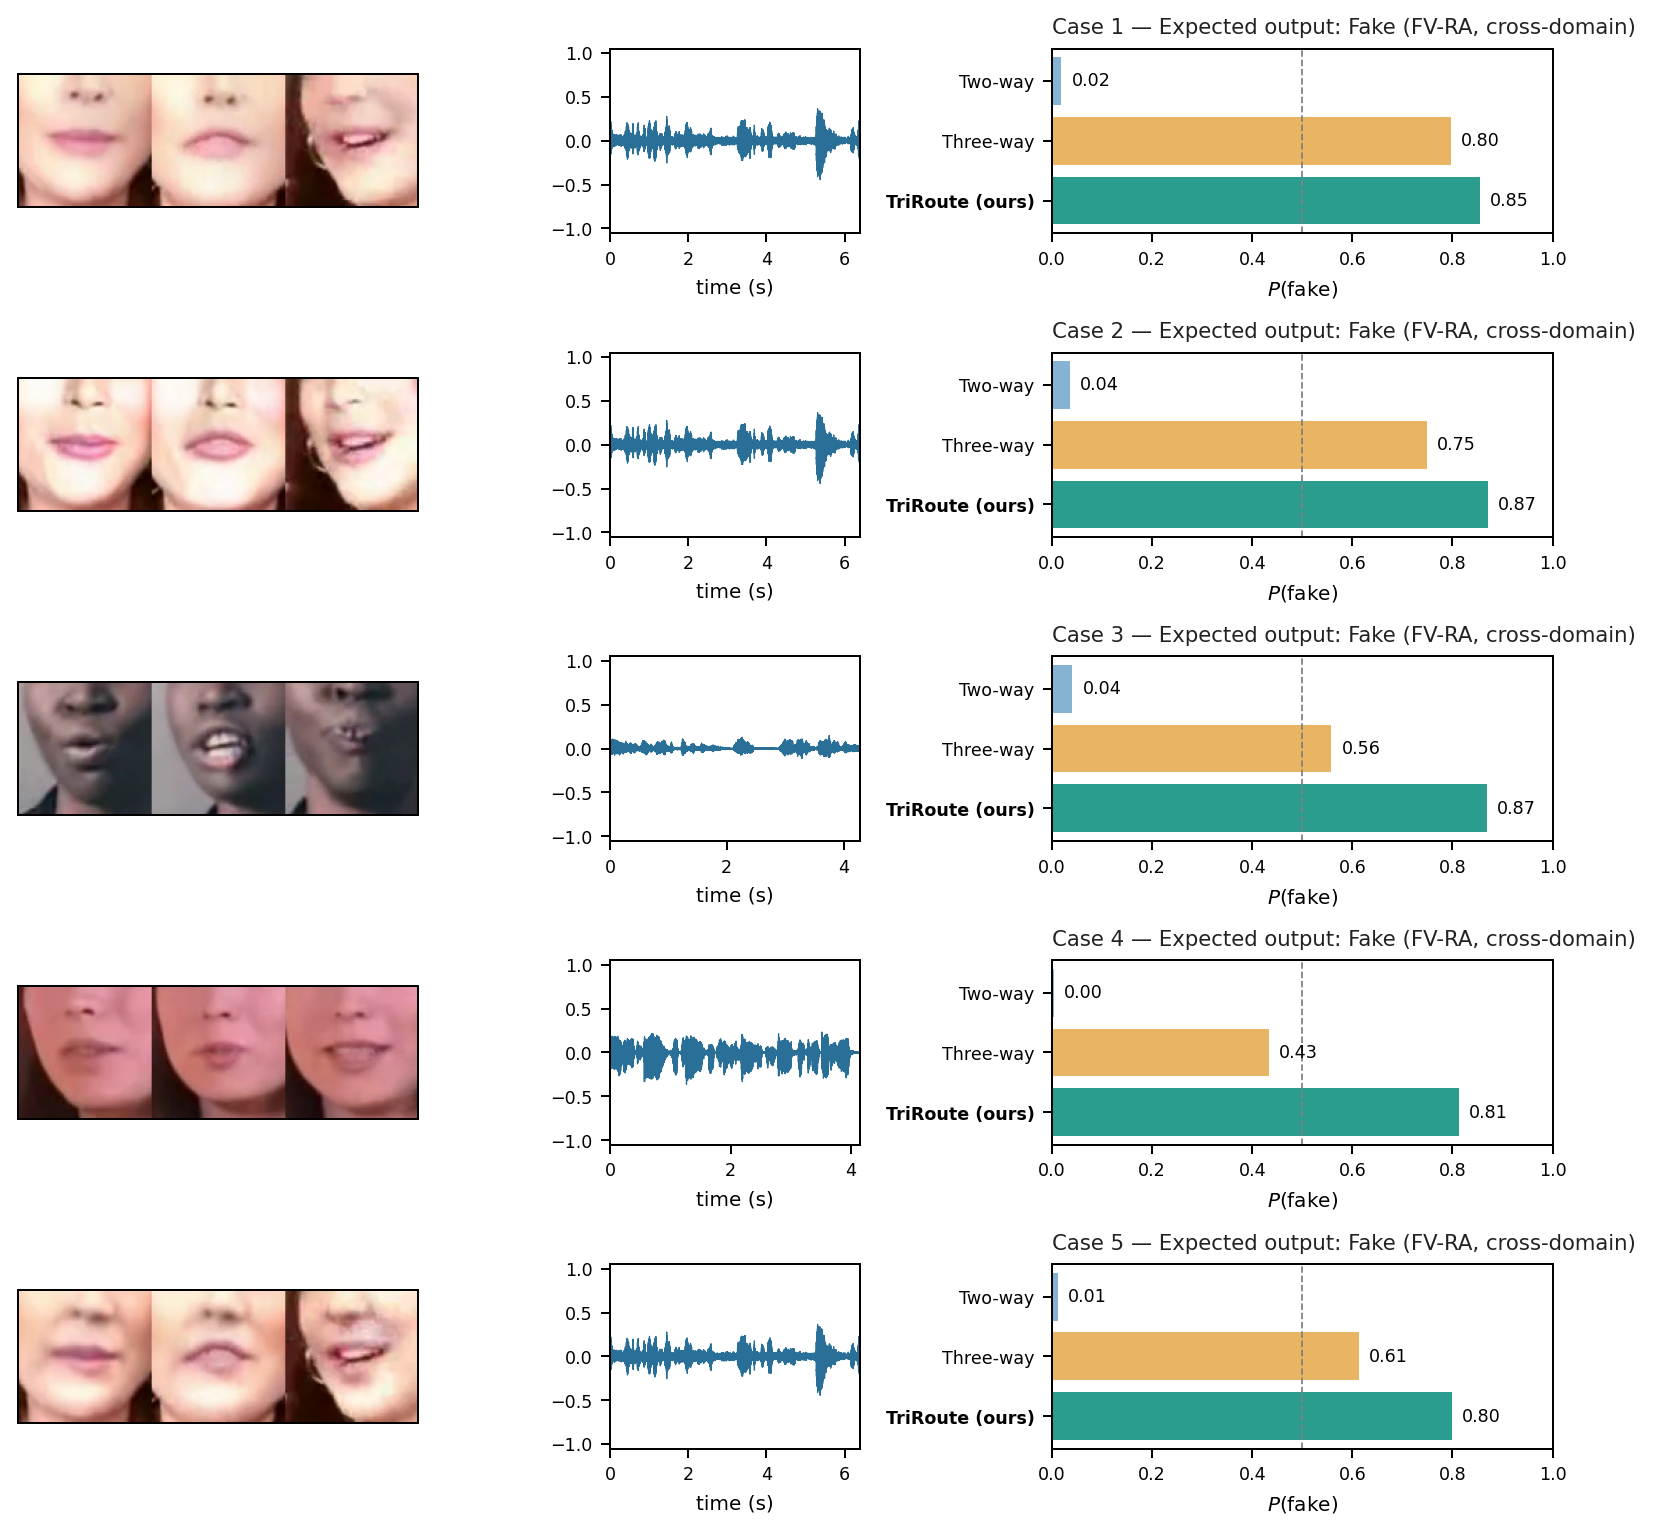
\includegraphics[width=0.92\linewidth]{figures/fig_qualitative_success_appendix.png}
    \caption{Additional FV-RA success cases where \method\ corrects the two-way baseline's audio-shortcut failure. For each row, \emph{left:} three lip-region frames; \emph{middle:} audio waveform; \emph{right:} model fake-probabilities. The two-way baseline assigns low fake probability, while \method\ assigns high fake probability.}
    \label{fig:qualitative_success_appendix}
\end{figure}

\begin{figure}[h]
    \centering
    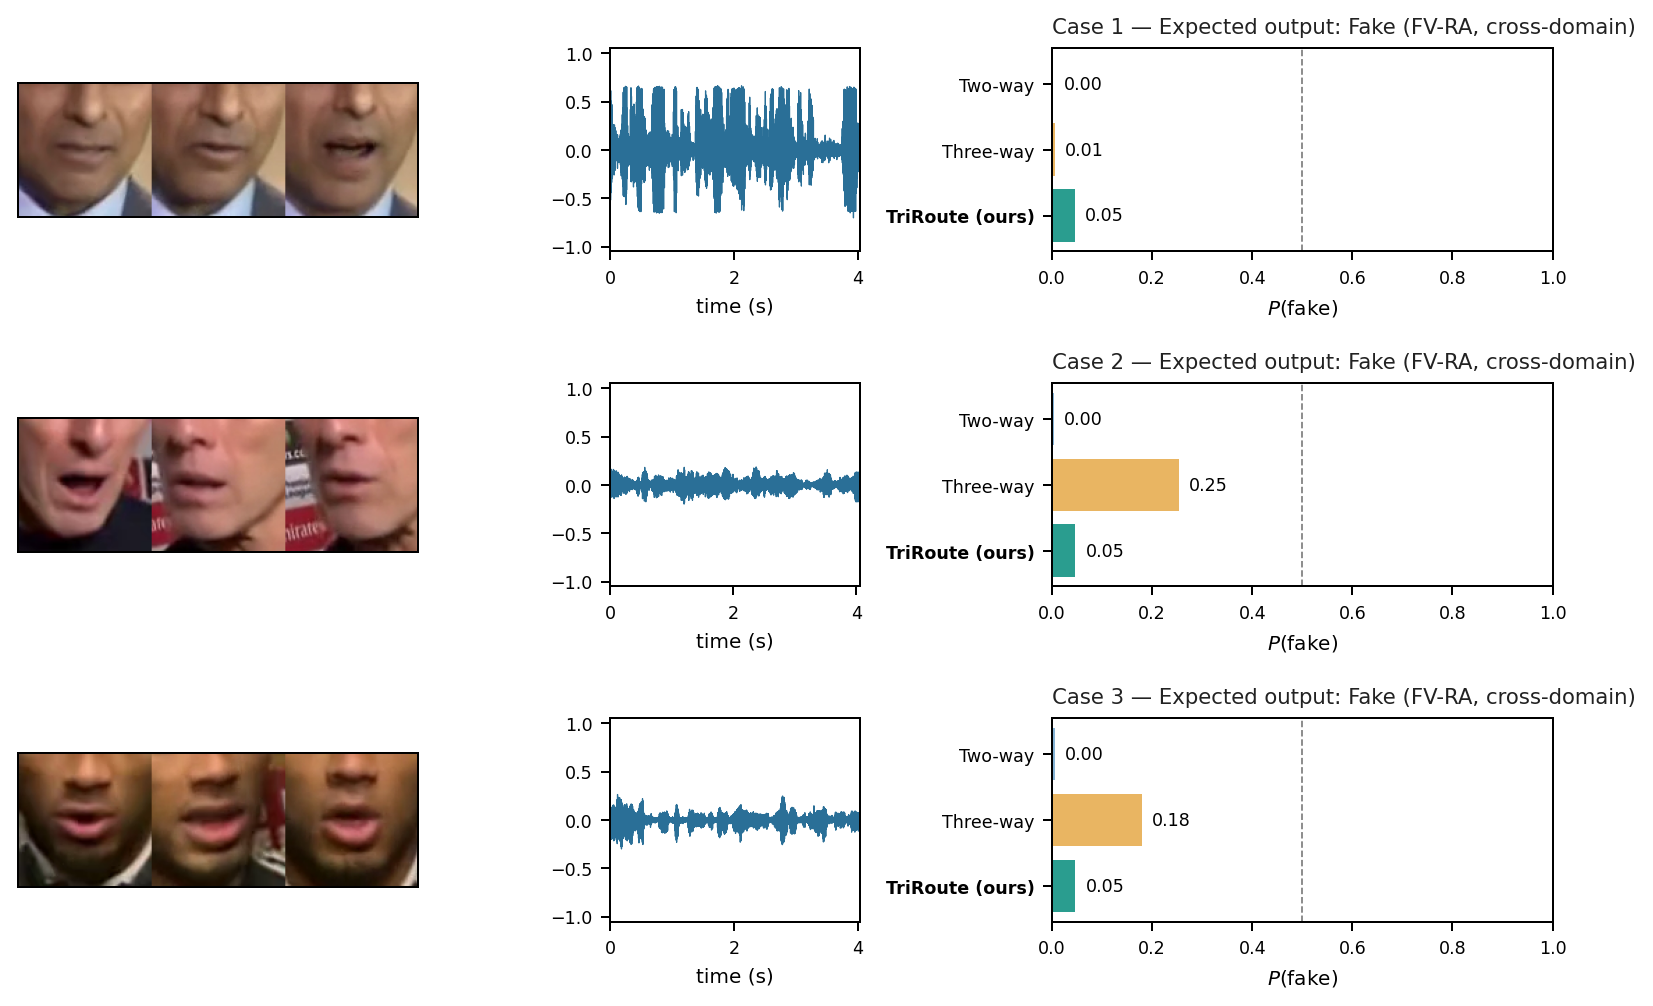
\includegraphics[width=0.92\linewidth]{figures/fig_qualitative_failure_appendix.png}
    \caption{FV-RA failure cases where \method\ remains confidently wrong. For each row, \emph{left:} three lip-region frames; \emph{middle:} audio waveform; \emph{right:} model fake-probabilities. These cases show that explicit routing substantially reduces the audio-shortcut failure mode but does not eliminate all difficult FV-RA errors.}
    \label{fig:qualitative_failure_appendix}
\end{figure}

\section{Unsupervised Scaling and Objective Stress Test}
\label{app:scaling_stress}

We tested whether simply increasing the amount of unsupervised pretraining data recovers the FV-RA routing behavior seen in \method. Table~\ref{tab:scaling_stress} reports FAVC AUC at peak epoch across two unsupervised training scales (120K and 250K clips). Performance saturates early and does not approach the FV-RA AUC achieved by structural factorization ($0.838$). These negative results support the main hypothesis: simply scaling unsupervised training or changing the objective does not recover the FV-RA routing behavior achieved by structural factorization. The bottleneck is routing structure, not data quantity.

\begin{table}[h]
    \centering
    \caption{Unsupervised scaling stress test on FAVC FV-RA AUC. Models are trained unsupervised at two data scales and evaluated at peak epoch. Neither scale closes the gap to the supervised \method\ result ($0.838$).}
    \label{tab:scaling_stress}
    \small
    \begin{tabular}{lccc}
        \toprule
        Training scale & Peak epoch & Best FAVC AUC & FV-RA AUC \\
        \midrule
        120k clips  & 16 & 0.931 & 0.854 \\
        250K clips  & 4 & 0.907 & 0.811 \\
        \midrule
        \method\ (our) & 68 & $0.922$ & $0.838$ \\
        \bottomrule
    \end{tabular}
    \vspace{0.5em}
\end{table}

\section{Post-Hoc Fusion Results}
\label{app:posthoc_fusion}

Table~\ref{tab:posthoc_fusion} reports the post-hoc fusion result moved from the main Table~8. This row combines the supervised \method\ detector with an unsupervised kNN anomaly score and is reported for completeness; it is not part of the headline comparison.

\begin{table}[h]
    \centering
    \caption{Post-hoc fusion: supervised \method\ + unsupervised kNN anomaly score, on FakeAVCeleb (FAVC) 70/30 test split and AV-Deepfake1M (AV1M) validation set. Values are percentages. Reported for completeness only; not a headline result.}
    \label{tab:posthoc_fusion}
    \resizebox{\linewidth}{!}{%
    \begin{tabular}{llllcccccccc}
        \toprule
        & & & & \multicolumn{4}{c}{Metric: AUC} & \multicolumn{4}{c}{Metric: AP} \\
        \cmidrule(lr){5-8}\cmidrule(lr){9-12}
        & & & & \multicolumn{2}{c}{FakeAVCeleb} & \multicolumn{2}{c}{AV-Deepfake1M} & \multicolumn{2}{c}{FakeAVCeleb} & \multicolumn{2}{c}{AV-Deepfake1M} \\
        \cmidrule(lr){5-6}\cmidrule(lr){7-8}\cmidrule(lr){9-10}\cmidrule(lr){11-12}
        Method & Mod. & Train type & Train data & Trim:$\times$ & Trim:$\checkmark$ & Trim:$\times$ & Trim:$\checkmark$ & Trim:$\times$ & Trim:$\checkmark$ & Trim:$\times$ & Trim:$\checkmark$ \\
        \midrule
        \quad + source-gated kNN & AV & post-hoc & AV1M & 95.7 & 92.8 & 99.6 & 85.4 & 99.9 & 99.8 & 99.7 & 93.7 \\
        \bottomrule
    \end{tabular}}
\end{table}

\section{Corrected Artifact Control}
\label{app:artifact_control}

A potential confound in AV1M-trained models is leading silence: fabricated clips sometimes begin with audio-free frames that are absent in authentic samples. We therefore evaluate a leading-silence-trimmed version that removes raw-waveform leading silence prior to AV-HuBERT feature extraction. Table~\ref{tab:silence_control_main} reports the trimming-induced change $\Delta = \mathrm{AUC}_{\mathrm{trimmed}} - \mathrm{AUC}_{\mathrm{untrimmed}}$ per category. The pattern is a stark asymmetry: RV-FA and FV-FA, the two audio-fake categories, drop by tens of AUC points after trimming, while FV-RA stays flat across every model ($|\Delta_\mathrm{FV\text{-}RA}| \le 0.008$). If the FV-RA gain were a leading-silence artifact, trimming would erase it. The fact that it does not means that FV-RA stability rules out audio shortcut explanations for the visual-routing gain. The trimming-induced drops are instead concentrated where they should be, in the audio-fake categories, indicating that the artifact mainly inflates audio-driven scoring. The full pre-/post-trim AUCs that produce these $\Delta$ values are reported in Table~\ref{tab:silence_control_full} in the appendix.

\begin{table}[t]
    \centering
    \caption{Trimming-induced change in AUC ($\Delta = \mathrm{trimmed} - \mathrm{untrimmed}$) on the FAVC categories, mean over three independent seeds. Audio-fake categories (RV-FA, FV-FA) drop substantially under trimming; FV-RA stays flat ($|\Delta| \le 0.008$) across all three models. Pre-/post-trim raw AUCs are deferred to Table~\ref{tab:silence_control_full} in the appendix.}
    \label{tab:silence_control_main}
    \small
    \begin{tabular}{lcc>{\columncolor[gray]{0.92}}cc}
        \toprule
        Model & $\Delta_\mathrm{Overall}$ & $\Delta_\mathrm{RV\text{-}FA}$ & $\Delta_\mathrm{FV\text{-}RA}$ (key) & $\Delta_\mathrm{FV\text{-}FA}$ \\
        \midrule
        Two-way baseline        & $-0.063$ & $-0.038$ & $\mathbf{-0.004}$ & $-0.141$ \\
        Three-way, no push-pull & $-0.050$ & $-0.049$ & $\mathbf{-0.008}$ & $-0.087$ \\
        \method\ (ours)         & $-0.056$ & $-0.189$ & $\mathbf{-0.005}$ & $-0.096$ \\
        \bottomrule
    \end{tabular}
\end{table}

\input{checklist}

\end{document}
